
\documentclass[11pt,aspectratio=169,xcolor=dvipsnames]{beamer}

% Impostazioni tema semplice e pulito
\usetheme{Boadilla}
\usecolortheme{default}
\setbeamertemplate{navigation symbols}{}

% 2. MODIFICA COLORI: Sostituisci blue!70!black con il colore scelto (es. MidnightBlue)
\setbeamercolor{title}{fg=PineGreen}
\setbeamercolor{frametitle}{fg=PineGreen}
\setbeamercolor{structure}{fg=PineGreen}
\setbeamerfont{frametitle}{series=\bfseries}

% Configurazione lingua e pacchetti
\usepackage[italian]{babel}
\usepackage[utf8]{inputenc}
\usepackage{graphicx}
\usepackage{amsmath}
\usepackage{booktabs}
% Dati per il frontespizio
\title{Progetto 2: Compressione di Immagini con DCT}
\subtitle{Metodi del Calcolo Scientifico}

% Tutti gli autori in un unico comando separati da \and
\author{Matias Bonoli \and Ashley Chudory \and Daniele Maccagnan}

\date{Anno accademico 2025/2026}

\begin{document}

\begin{frame}[plain]
    \titlepage
\end{frame}

\begin{frame}{Introduzione al Progetto}
    L'obiettivo è studiare e applicare la Trasformata Discreta del Coseno (DCT) per la compressione di immagini in toni di grigio. Il lavoro si divide in due fasi:
    \begin{itemize}
        \item Implementazione della DCT bidimensionale: scrittura di una versione basata sul prodotto matriciale e confronto con l'implementazione \emph{fast} di libreria.
        \item Sviluppo di un software con interfaccia grafica per applicare la compressione a blocchi su immagini reali e sintetiche.
        \item Analisi del compromesso tra compressione e qualità al variare della dimensione dei blocchi ($F$) e della soglia di taglio delle alte frequenze ($d$).
    \end{itemize}
\end{frame}

\begin{frame}{La Trasformata Discreta del Coseno (DCT)}
    La DCT nasce dalla teoria delle serie di Fourier per approssimare un segnale campionato riducendo il fenomeno di Gibbs ai bordi.
    \begin{itemize}
        \item Il segnale viene riflesso per renderlo pari, per poi periodizzarlo: si eliminano così le discontinuità e si azzerano i coefficienti associati ai seni, lasciando una base di soli coseni ortogonali.
        \item Compattazione dell'energia: più l'immagine è liscia, più i coefficienti della trasformata decadono rapidamente all'aumentare delle frequenze.
        \item La DCT concentra quasi tutta l'energia a bassa frequenza, permettendo di azzerare quelle alte con un degrado visivo minimo.
    \end{itemize}
\end{frame}

\begin{frame}{DCT2: Implementazione Custom}
    Abbiamo sfruttato la \emph{separabilità} del nucleo coseno.
    \begin{itemize}
        \item Costruzione esplicita della matrice ortonormale di trasformazione $D \in \mathbb{R}^{N \times N}$.
        \item Trasformata applicata prima alle colonne e poi alle righe: $D \cdot f \cdot D^\top$.
        \item Essendo due moltiplicazioni dense, il costo asintotico è $O(N^3)$.
    \end{itemize}
\end{frame}

\begin{frame}{DCT2: Implementazione Fast}
    \begin{itemize}
        \item Utilizzo delle funzioni di libreria \texttt{scipy.fft.dctn} e \texttt{idctn}.
        \item Sfrutta l'algoritmo FFT (\textit{Fast Fourier Transform}), riducendo il costo a $O(N^2 \log N)$.
        \item Parametri usati: \texttt{type=2} e \texttt{norm="ortho"}.
        \item Risultati confrontabili (stessa base ortonormale) con la versione custom.
    \end{itemize}
\end{frame}

\begin{frame}{Validazione del calcolo}
    Test eseguiti sui blocchi $1\times 8$ e $8\times 8$ della traccia:
    \begin{itemize}
        \item Le versioni custom e fast coincidono a meno della precisione di macchina (errore $\sim 10^{-13}$).
        \item L'errore sulla terza cifra decimale rispetto alla traccia è dovuto all'arrotondamento dei valori forniti.
        \item La ricostruzione $\mathrm{IDCT2}(\mathrm{DCT2}(A)) = A$ risulta accurata a meno di $10^{-13}$.
    \end{itemize}
\end{frame}

\begin{frame}{Confronto dei Tempi}
    \begin{figure}
        \centering
        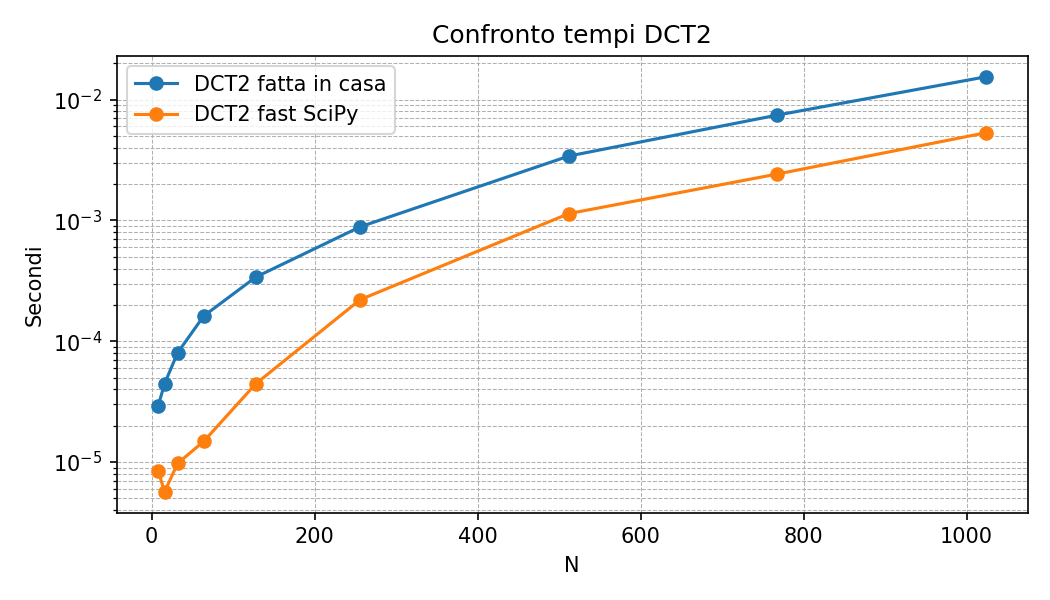
\includegraphics[width=\textwidth,height=0.85\textheight,keepaspectratio]{../relazione/figures/benchmark_dct2.png}
    \end{figure}
\end{frame}


% ===============================
% PARTE 2: ALGORITMO E GUI
% ===============================
\section{Parte 2: Algoritmo di Compressione}

\begin{frame}{L'algoritmo di compressione}
    \begin{enumerate}
        \item Divisione dell'immagine in blocchi quadrati $F \times F$.
        \item Passaggio al dominio delle frequenze tramite la trasformata DCT2.
        \item Azzeramento delle frequenze alte ponendo a zero i coefficienti con $k + \ell \ge d$.
        \item Ritorno al dominio dei pixel applicando la trasformata inversa IDCT2.
        \item Arrotondamento dei pixel in $[0, 255]$ e ricomposizione dell'immagine finale.
    \end{enumerate}
\end{frame}

\begin{frame}{Setup Sperimentale}
    \begin{itemize}
        \item Interfaccia in \texttt{tkinter} per testare parametri $F$ e $d$ con validazione in tempo reale ($0 \le d \le 2F-2$).
        \item Testate 12 configurazioni per immagine incrociando le dimensioni dei blocchi con soglie crescenti.
        \item Analisi condotta su blocchi quadrati di dimensione $F \in \{8, 16, 32\}$.
        \item Studio dell'effetto del taglio $d$ e dell'impatto della dimensione del blocco $F$.
    \end{itemize}
\end{frame}

% ===============================
% ESPERIMENTI: IMMAGINI SINTETICHE
% ===============================
\section{Esperimenti}

\begin{frame}{Gradiente Orizzontale: Analisi}
    \begin{itemize}
        \item Rappresenta il caso d'uso ideale per la compressione DCT.
        \item L'intensità risulta graduale lungo un'unica direzione.
        \item L'energia si concentra quasi tutta nel coefficiente $c_{0,0}$ e nel primo coefficiente direzionale.
        \item L'azzeramento delle alte frequenze lascia l'immagine inalterata.
    \end{itemize}
\end{frame}

\begin{frame}{Gradiente Orizzontale: Risultati}
    \begin{itemize}
        \item La ricostruzione appare visivamente indistinguibile dall'originale.
        \item Con $d=2$ (meno del $5\%$ dei coefficienti) il PSNR supera agilmente i $54$~dB.
        \item Aumentare $d$ non porta miglioramenti in quanto l'errore si annulla già a soglie minime.
        \item Si ottiene una compressione ottimale con un azzeramento massiccio ma senza alcuna perdita percepibile.
    \end{itemize}
\end{frame}

\begin{frame}{Gradiente Liscio -- Originale}
    \begin{figure}
        \centering
        
\includegraphics[width=\textwidth,height=0.85\textheight,keepaspectratio]{../relazione/figures/orig_gradient.png}
    \end{figure}
\end{frame}

\begin{frame}{Gradiente Liscio -- Griglia delle ricostruzioni}
    \begin{figure}
        \centering
        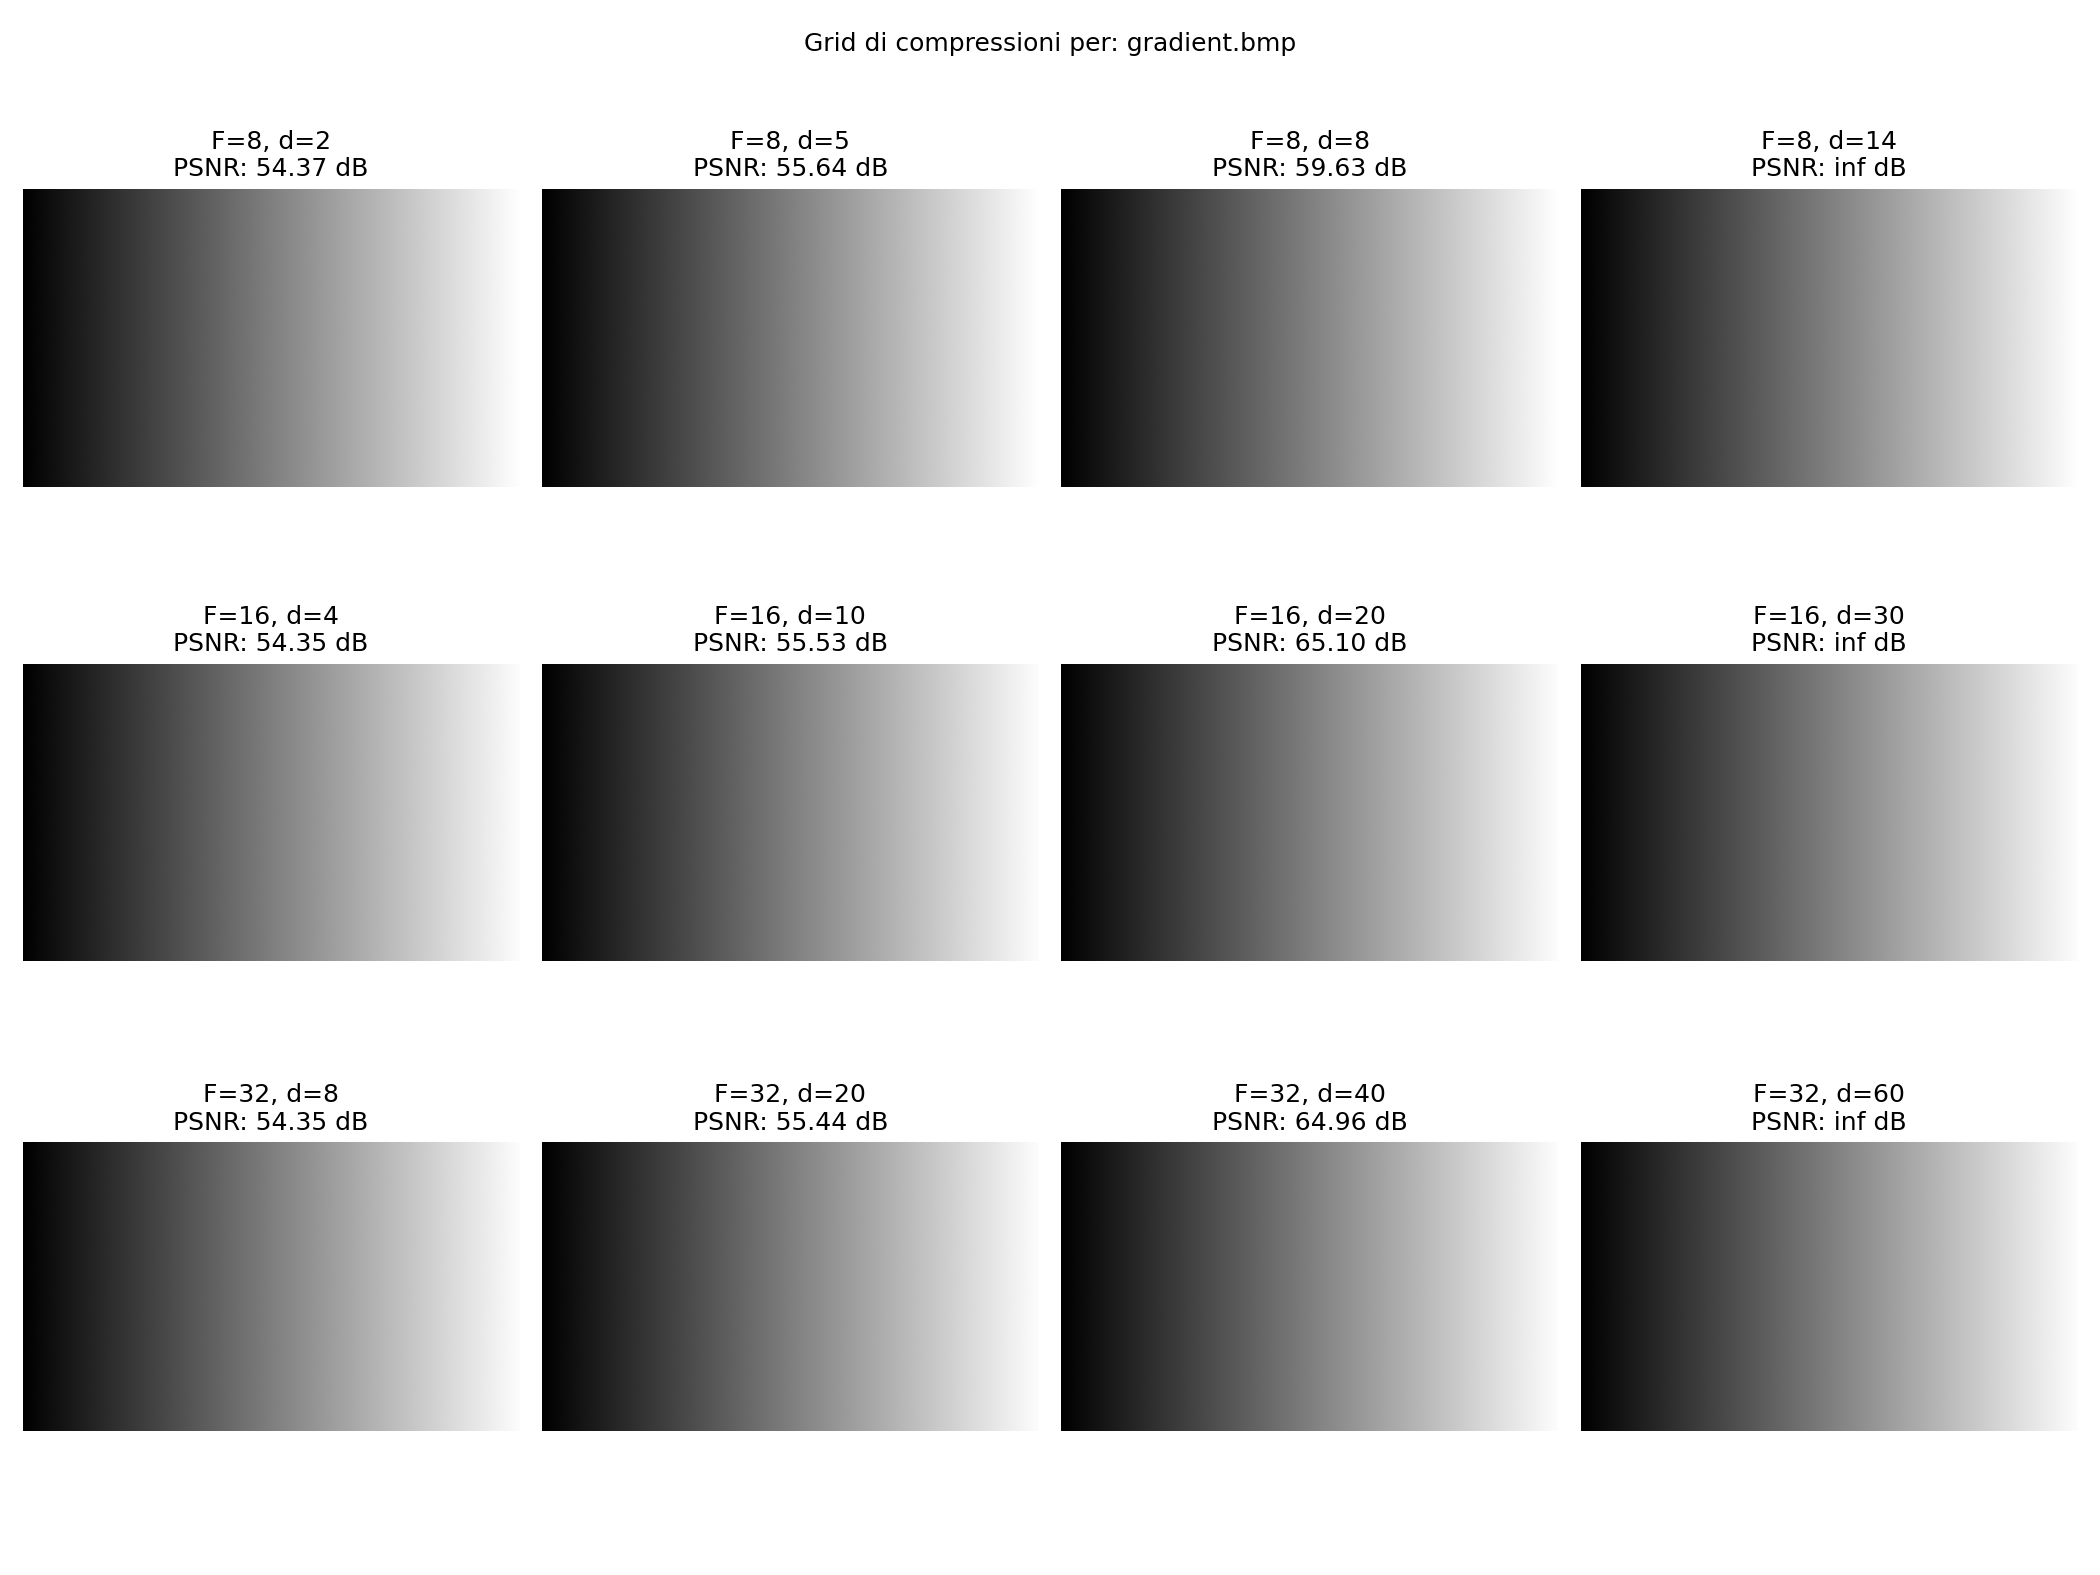
\includegraphics[width=\textwidth,height=0.85\textheight,keepaspectratio]{../relazione/figures/gradient_grid.png}
    \end{figure}
\end{frame}

\begin{frame}{Gradiente Liscio -- PSNR e Metriche}
    \begin{figure}
        \centering
        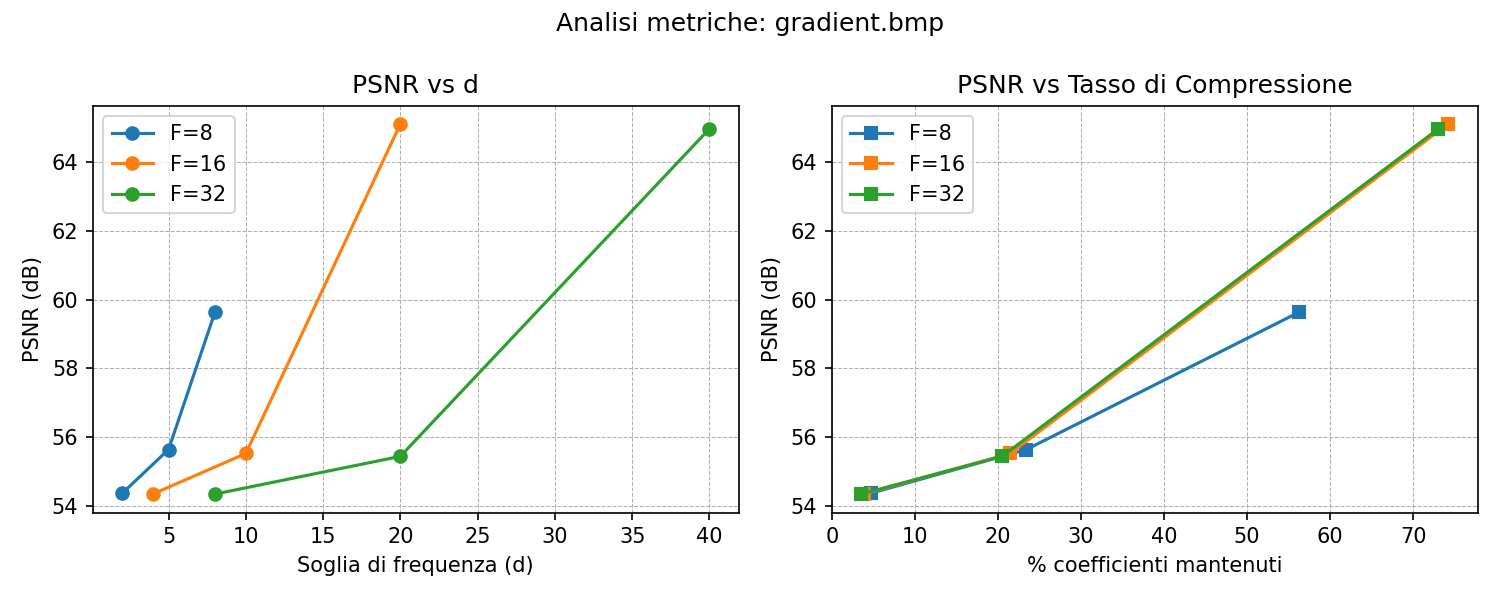
\includegraphics[width=\textwidth,height=0.85\textheight,keepaspectratio]{../relazione/figures/gradient_metrics.png}
    \end{figure}
\end{frame}

\begin{frame}{Carattere a contrasto pieno: Analisi}
    \begin{itemize}
        \item L'immagine presenta pochi bordi netti ad alto contrasto ed è priva di texture fini.
        \item Costituisce il caso antitetico al gradiente ed è ideale per osservare il fenomeno di Gibbs.
        \item L'informazione dei contorni non è concentrata ma risulta distribuita su un ampio spettro.
        \item L'azzeramento delle alte frequenze crea immediatamente artefatti e aloni.
    \end{itemize}
\end{frame}

\begin{frame}{Carattere a contrasto pieno: Risultati}
    \begin{itemize}
        \item A soglie basse ($d \in [2,8]$) il PSNR resta tra $17$ e $27$~dB causando un evidente alone chiaro.
        \item La qualità torna soddisfacente solo a valori di $d$ massimi reintroducendo le transizioni nette.
        \item A parità di coefficienti mantenuti i blocchi più ampi performano meglio.
        \item Con $F=32$ si raggiungono $31$~dB mentre con $F=8$ ci si ferma a $27$~dB in quanto il blocco esteso modella meglio il contorno.
    \end{itemize}
\end{frame}

\begin{frame}{Carattere a Contrasto pieno: Originale}
    \begin{figure}
        \centering
        
\includegraphics[width=\textwidth,height=0.85\textheight,keepaspectratio]{../relazione/figures/orig_prova.png}
    \end{figure}
\end{frame}

\begin{frame}{Carattere a Contrasto pieno: Griglia delle ricostruzioni}
    \begin{figure}
        \centering
        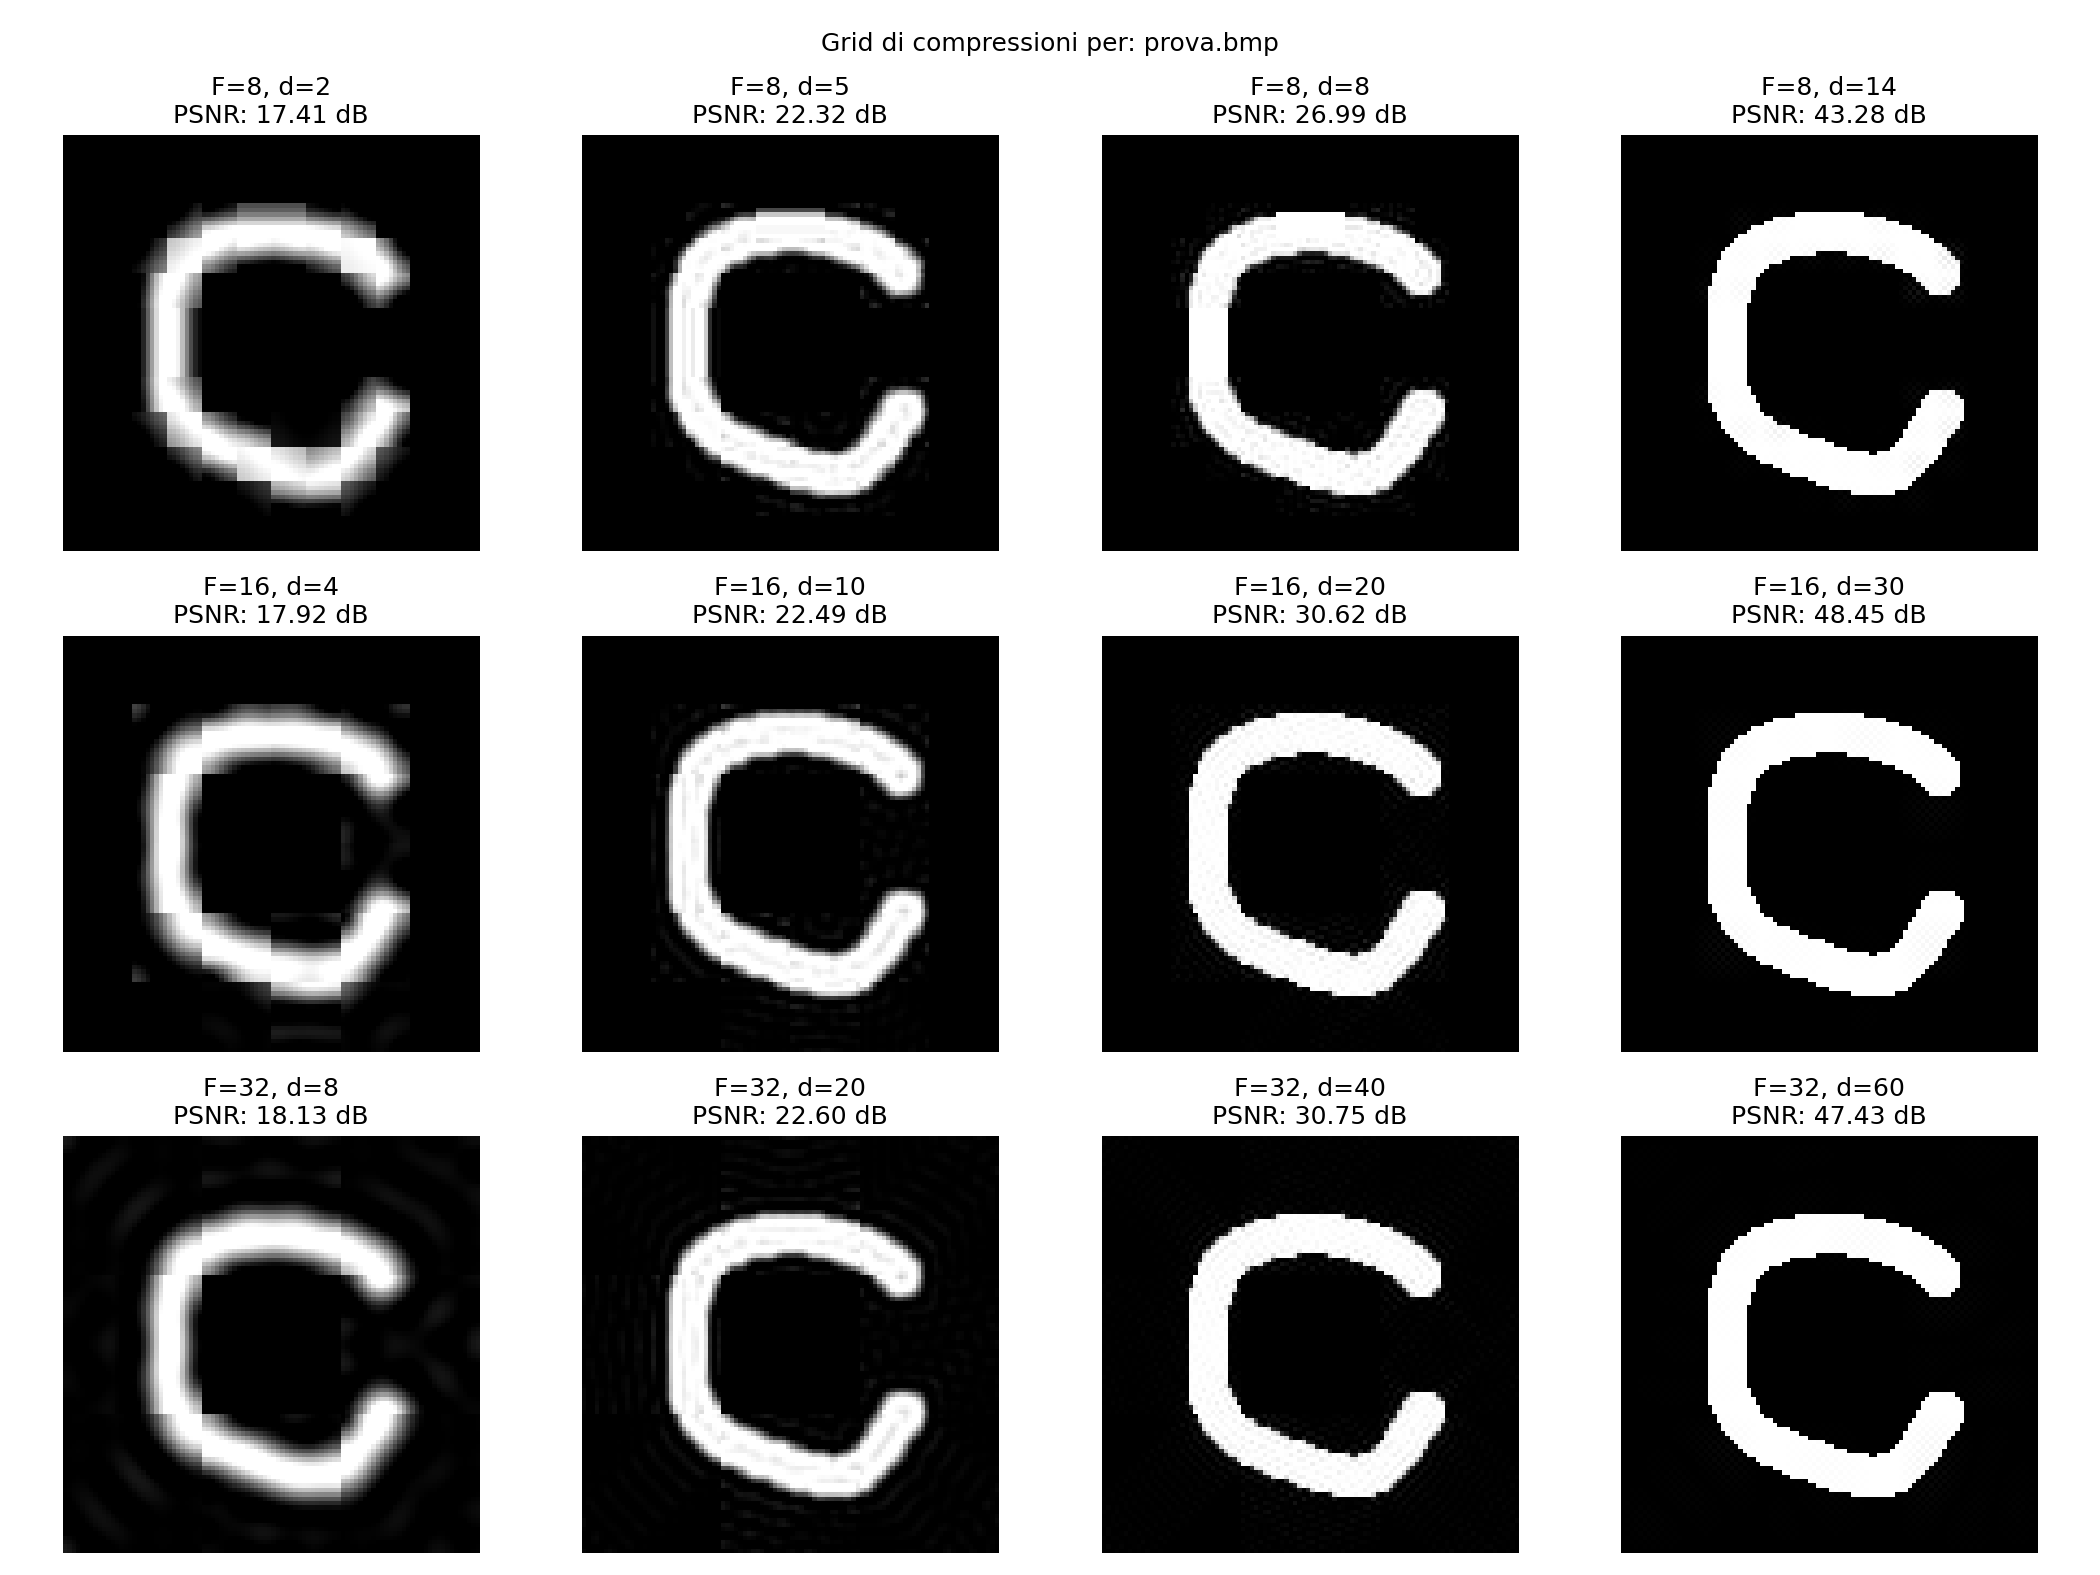
\includegraphics[width=\textwidth,height=0.85\textheight,keepaspectratio]{../relazione/figures/prova_grid.png}
    \end{figure}
\end{frame}

\begin{frame}{Carattere a Contrasto pieno: PSNR e Metriche}
    \begin{figure}
        \centering
        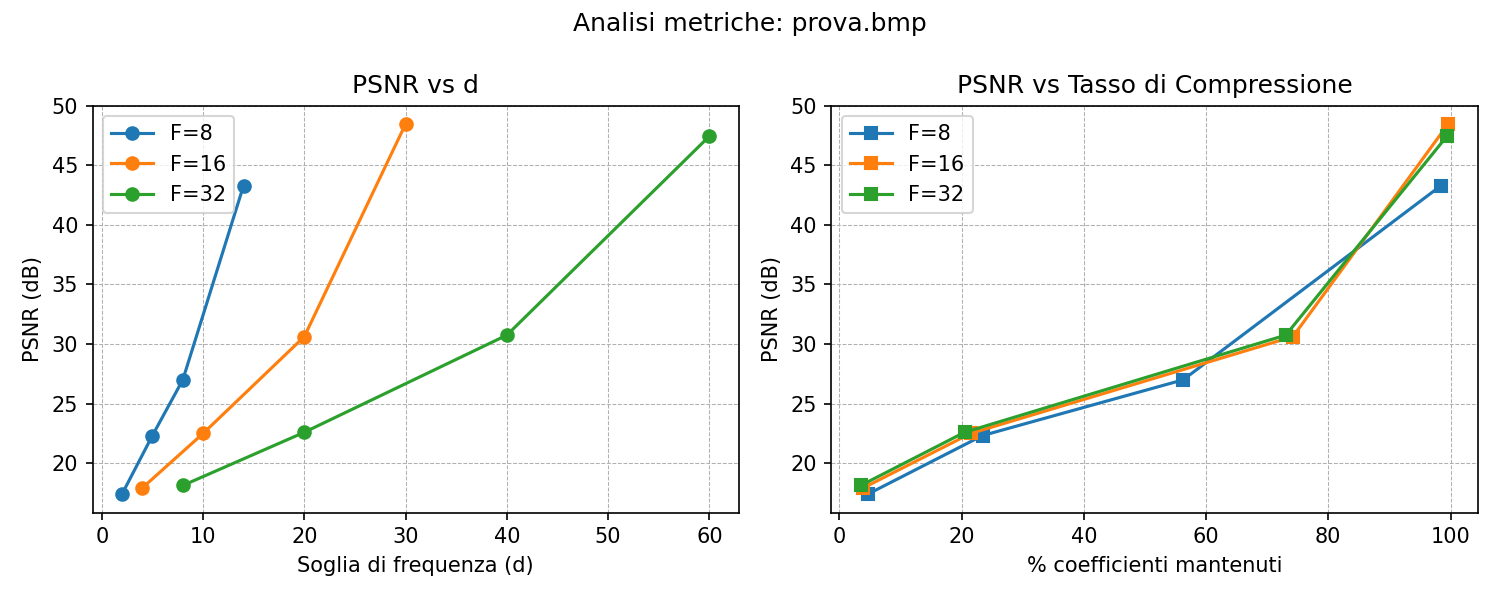
\includegraphics[width=\textwidth,height=0.85\textheight,keepaspectratio]{../relazione/figures/prova_metrics.png}
    \end{figure}
\end{frame}

\begin{frame}{Alta frequenza densa: La Scacchiera (Analisi)}
    \begin{itemize}
        \item Rappresenta lo scenario in assoluto più ostico per la compressione DCT.
        \item Il pattern è un'alternanza periodica di celle $10 \times 10$ con continue transizioni nette da $0$ a $255$.
        \item I continui bordi ripetuti spostano in modo deciso lo spettro verso le alte frequenze.
        \item La maschera di taglio ($k+\ell < d$) scarta in questo caso proprio l'informazione essenziale.
    \end{itemize}
\end{frame}

\begin{frame}{Alta frequenza densa: La Scacchiera (Risultati)}
    \begin{itemize}
        \item A soglie basse si assiste a un repentino crollo del PSNR sotto i $18$~dB.
        \item Tagliando le frequenze resta solo la media d'intensità trasformando l'immagine in tasselli grigi.
        \item La struttura originaria viene ripristinata solo con valori di $d$ molto elevati rinunciando alla compressione.
        \item Le celle e i blocchi si sincronizzano a intervalli regolari rendendo identici i risultati su scacchiere multiple di quel lato.
    \end{itemize}
\end{frame}

\begin{frame}{Scacchiera 20x20: Originale}
    \begin{figure}
        \centering
        
\includegraphics[width=\textwidth,height=0.85\textheight,keepaspectratio]{../relazione/figures/orig_20x20.png}
    \end{figure}
\end{frame}

\begin{frame}{Scacchiera 20x20: Griglia delle ricostruzioni}
    \begin{figure}
        \centering
        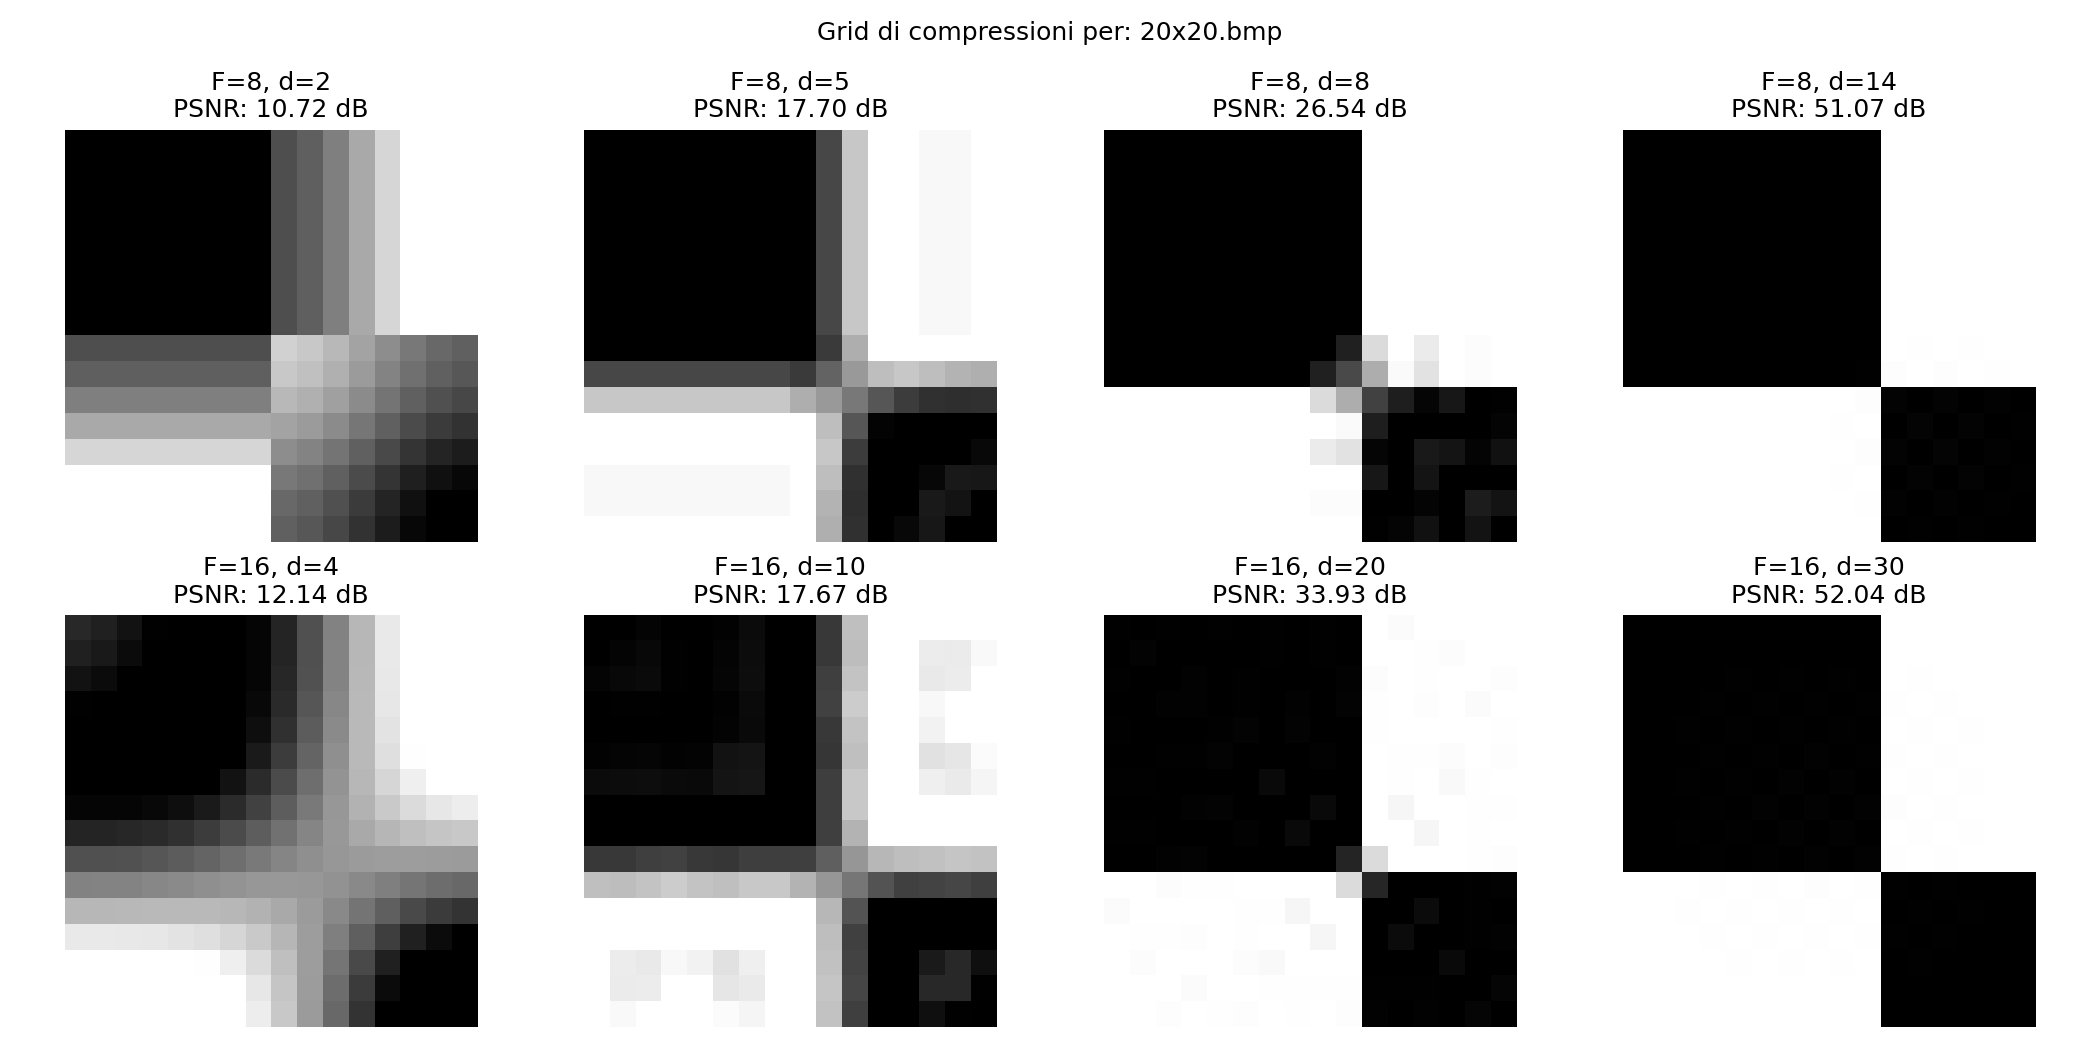
\includegraphics[width=\textwidth,height=0.85\textheight,keepaspectratio]{../relazione/figures/20x20_grid.png}
    \end{figure}
\end{frame}

\begin{frame}{Scacchiera 20x20: PSNR e Metriche}
    \begin{figure}
        \centering
        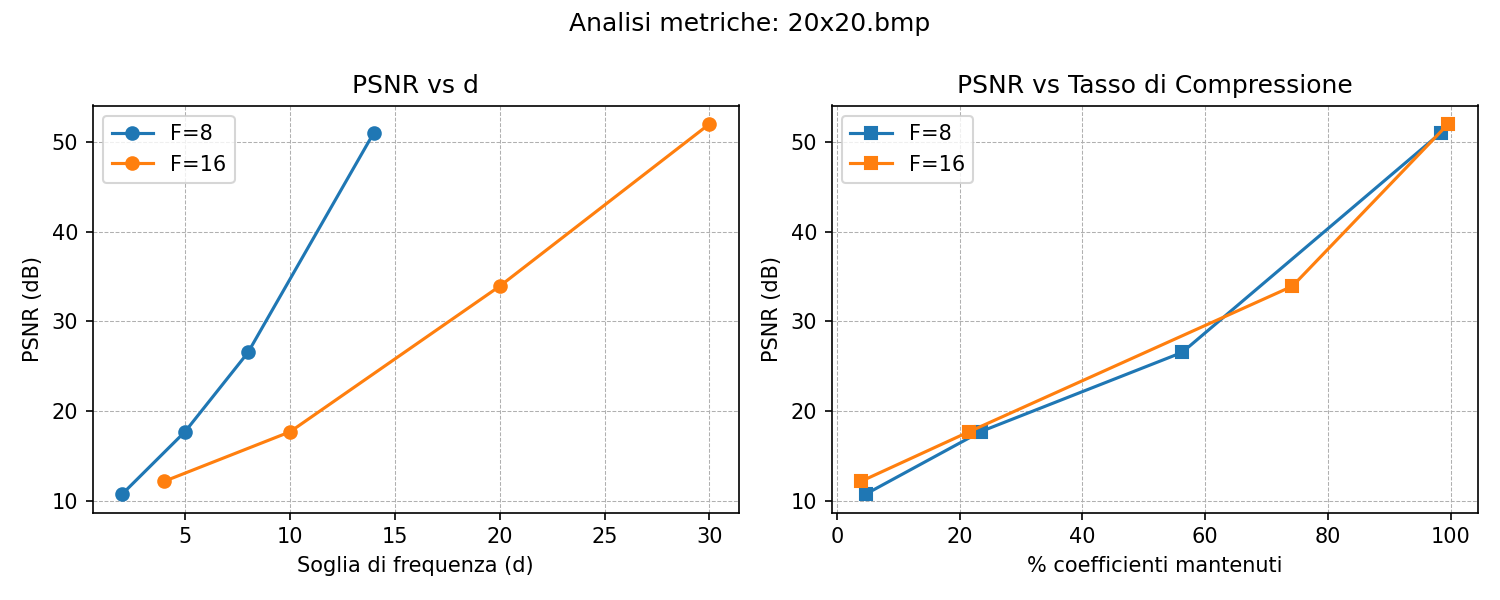
\includegraphics[width=\textwidth,height=0.85\textheight,keepaspectratio]{../relazione/figures/20x20_metrics.png}
    \end{figure}
\end{frame}

\begin{frame}{Scacchiera 160x160: Originale}
    \begin{figure}
        \centering
        
\includegraphics[width=\textwidth,height=0.85\textheight,keepaspectratio]{../relazione/figures/orig_160x160.png}
    \end{figure}
\end{frame}

\begin{frame}{Scacchiera 160x160: Griglia delle ricostruzioni}
    \begin{figure}
        \centering
        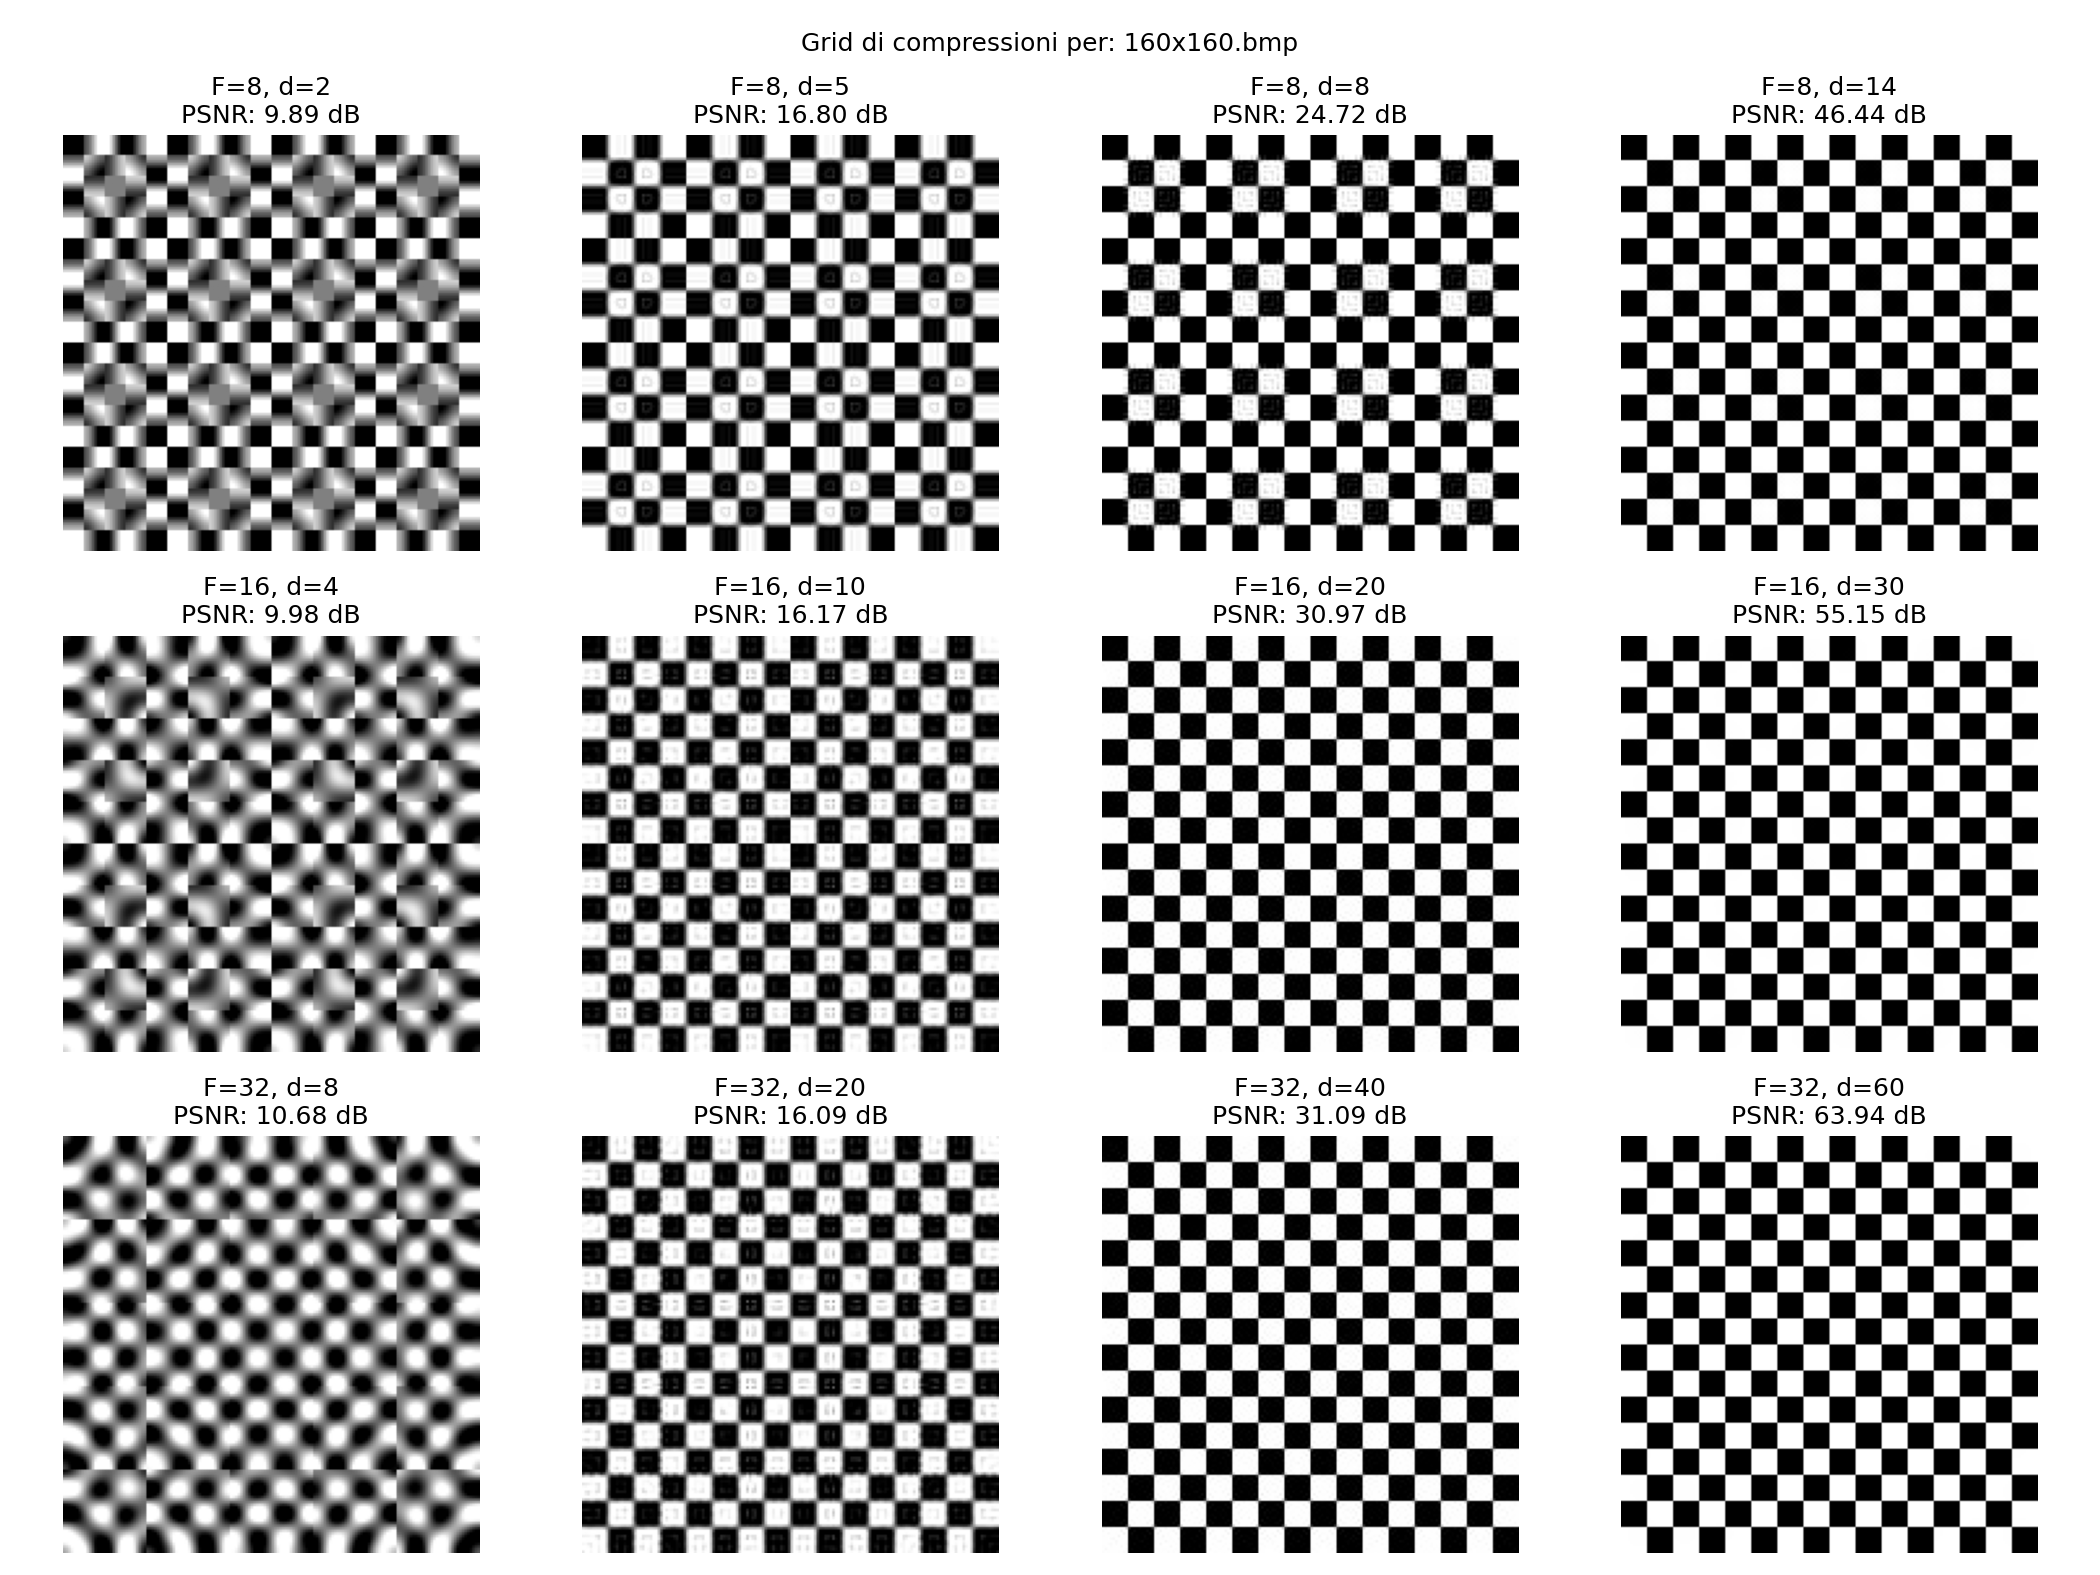
\includegraphics[width=\textwidth,height=0.85\textheight,keepaspectratio]{../relazione/figures/160x160_grid.png}
    \end{figure}
\end{frame}

\begin{frame}{Scacchiera 160x160: PSNR e Metriche}
    \begin{figure}
        \centering
        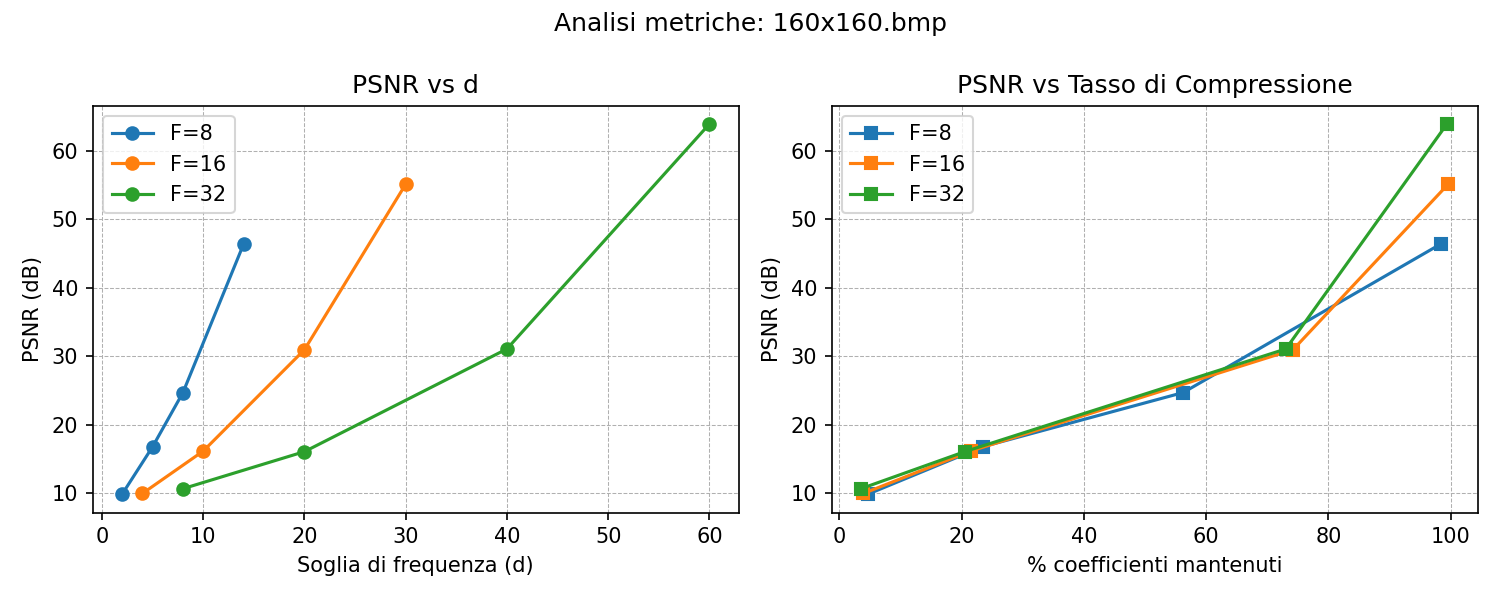
\includegraphics[width=\textwidth,height=0.85\textheight,keepaspectratio]{../relazione/figures/160x160_metrics.png}
    \end{figure}
\end{frame}

\begin{frame}{Scacchiera 640x640: Originale}
    \begin{figure}
        \centering
        
\includegraphics[width=\textwidth,height=0.85\textheight,keepaspectratio]{../relazione/figures/orig_640x640.png}
    \end{figure}
\end{frame}

\begin{frame}{Scacchiera 640x640: Griglia delle ricostruzioni}
    \begin{figure}
        \centering
        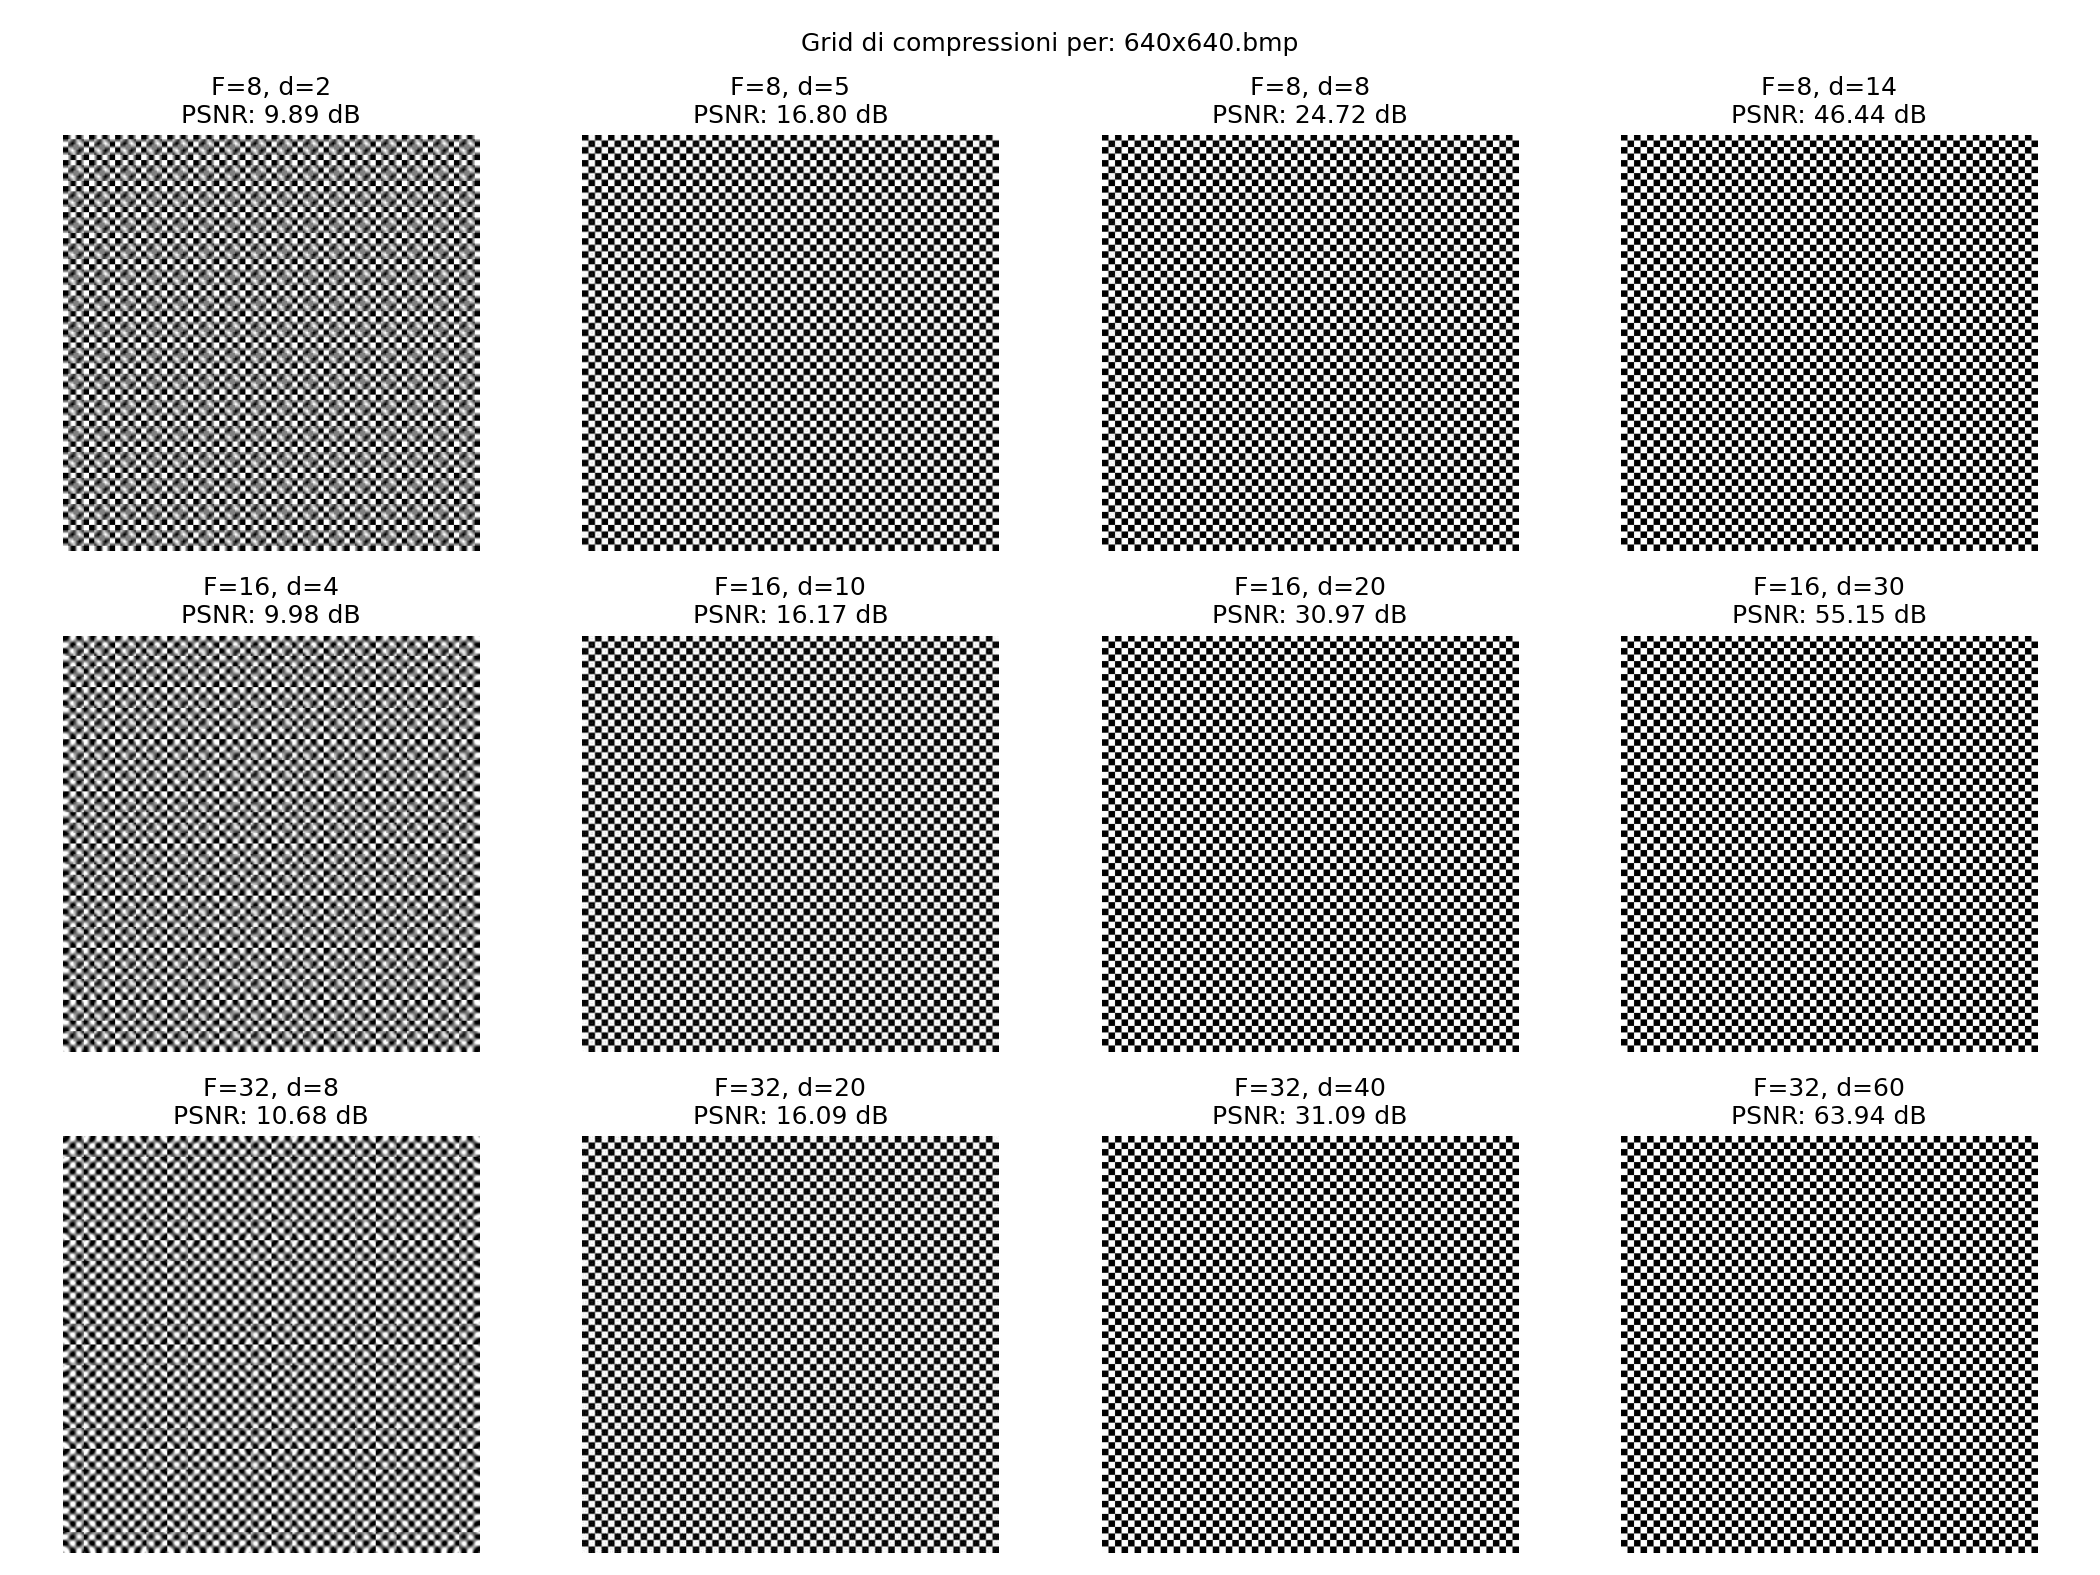
\includegraphics[width=\textwidth,height=0.85\textheight,keepaspectratio]{../relazione/figures/640x640_grid.png}
    \end{figure}
\end{frame}

\begin{frame}{Scacchiera 640x640: PSNR e Metriche}
    \begin{figure}
        \centering
        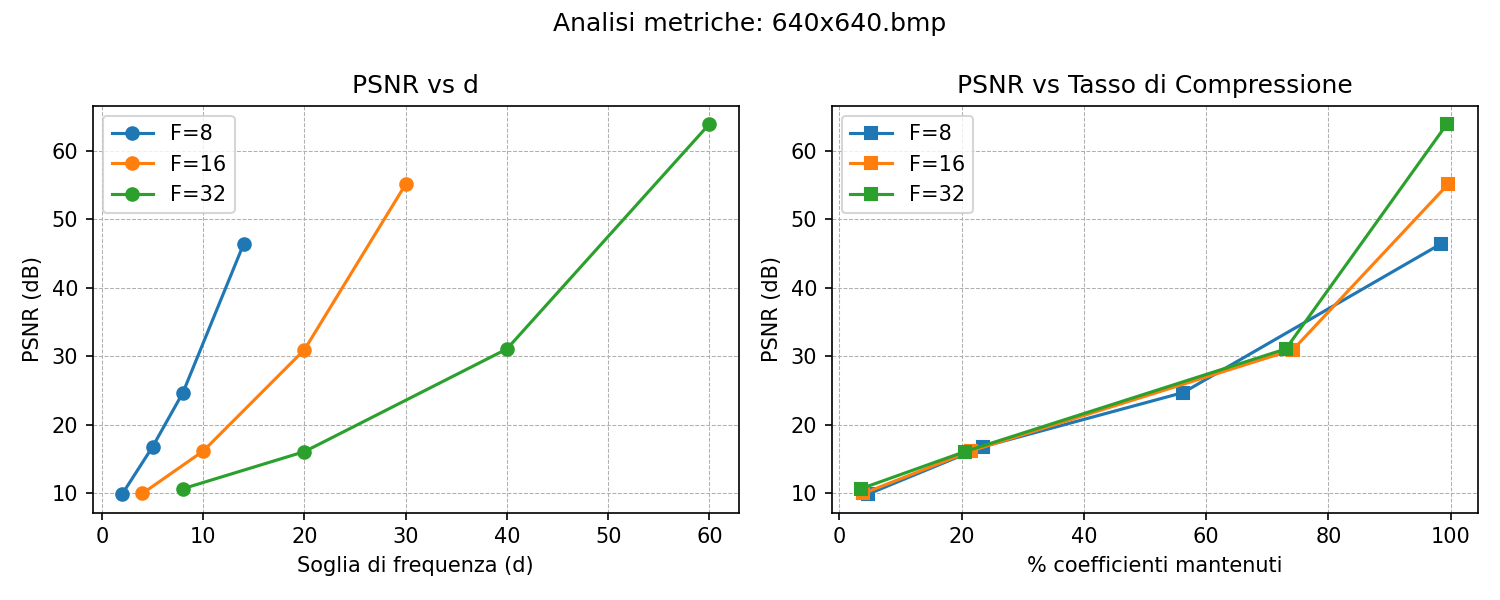
\includegraphics[width=\textwidth,height=0.85\textheight,keepaspectratio]{../relazione/figures/640x640_metrics.png}
    \end{figure}
\end{frame}

\begin{frame}{Scacchiera: Il caso limite F=10}
    \begin{itemize}
        \item Impostando la dimensione del blocco a $F=10$, si ottiene un allineamento spaziale perfetto con le celle $10 \times 10$ dell'immagine.
        \item Ogni blocco ricade interamente all'interno di una singola cella, presentando così pixel di intensità del tutto uniforme.
        \item L'energia spaziale si concentra unicamente nella componente continua, permettendo una compressione perfetta al minimo della soglia.
    \end{itemize}
\end{frame}

\begin{frame}{Scacchiera 20x20: Compressione con F=10}
    \begin{figure}
        \centering
        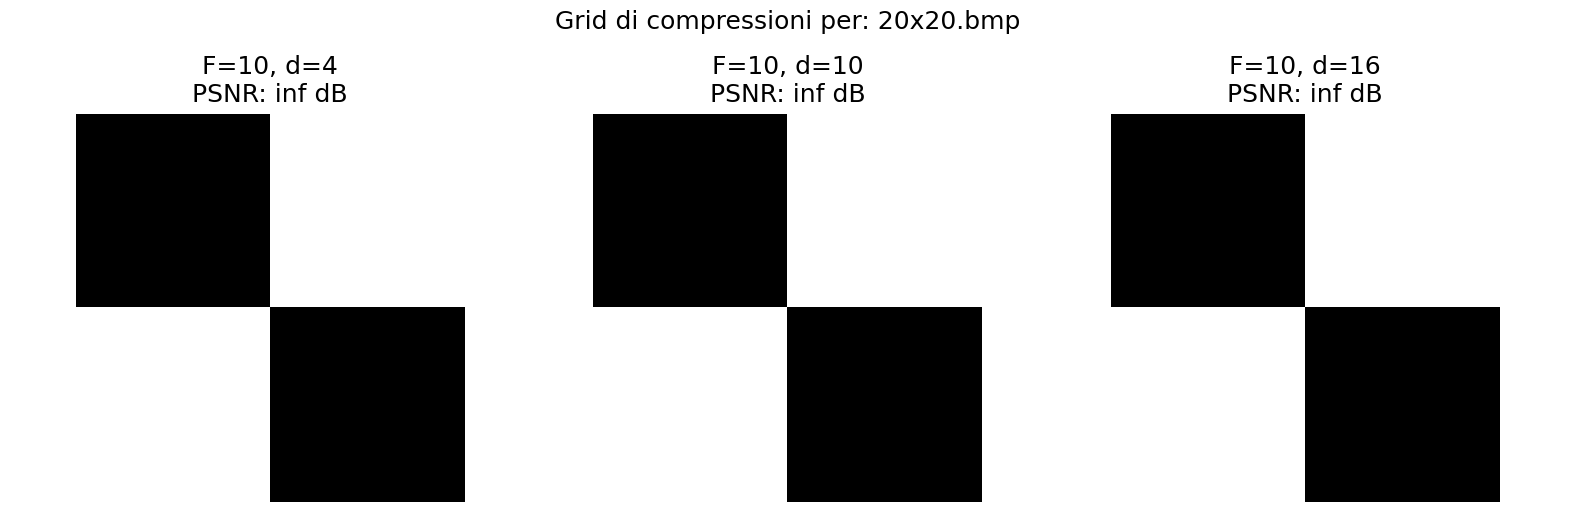
\includegraphics[width=\textwidth,height=0.85\textheight,keepaspectratio]{../relazione/figures/20x20_grid_F10.png}
    \end{figure}
\end{frame}

\begin{frame}{Scacchiera 160x160: Compressione con F=10}
    \begin{figure}
        \centering
        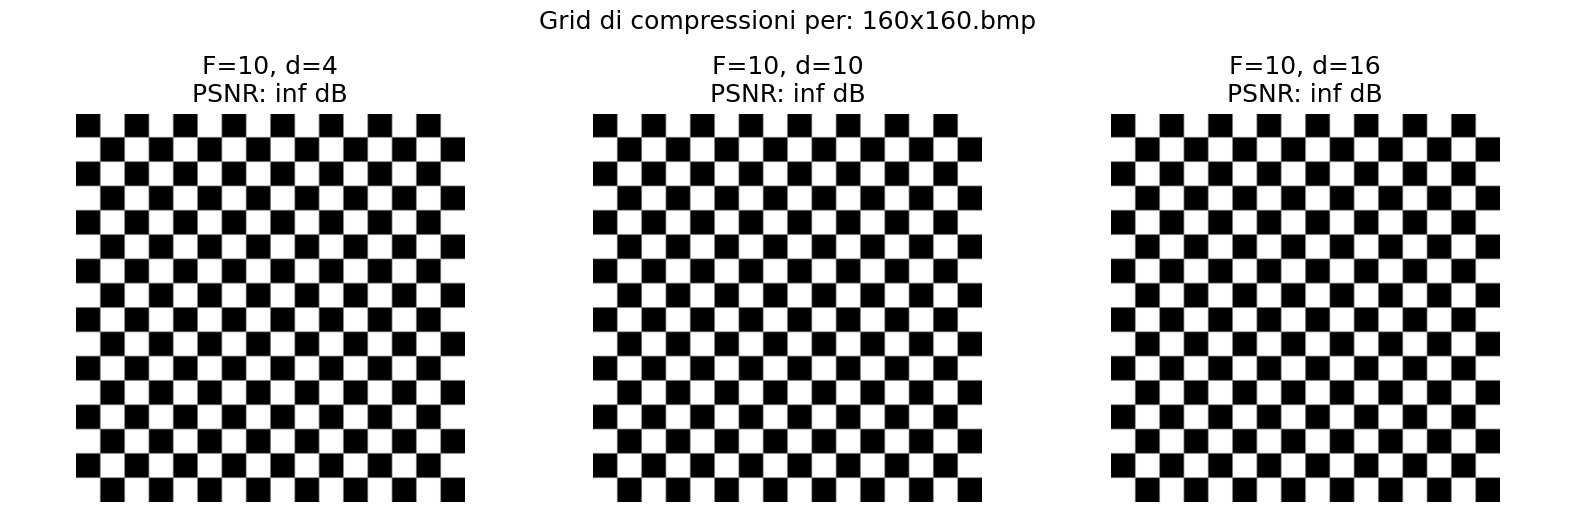
\includegraphics[width=\textwidth,height=0.85\textheight,keepaspectratio]{../relazione/figures/160x160_grid_F10.png}
    \end{figure}
\end{frame}

\begin{frame}{Scacchiera 640x640: Compressione con F=10}
    \begin{figure}
        \centering
        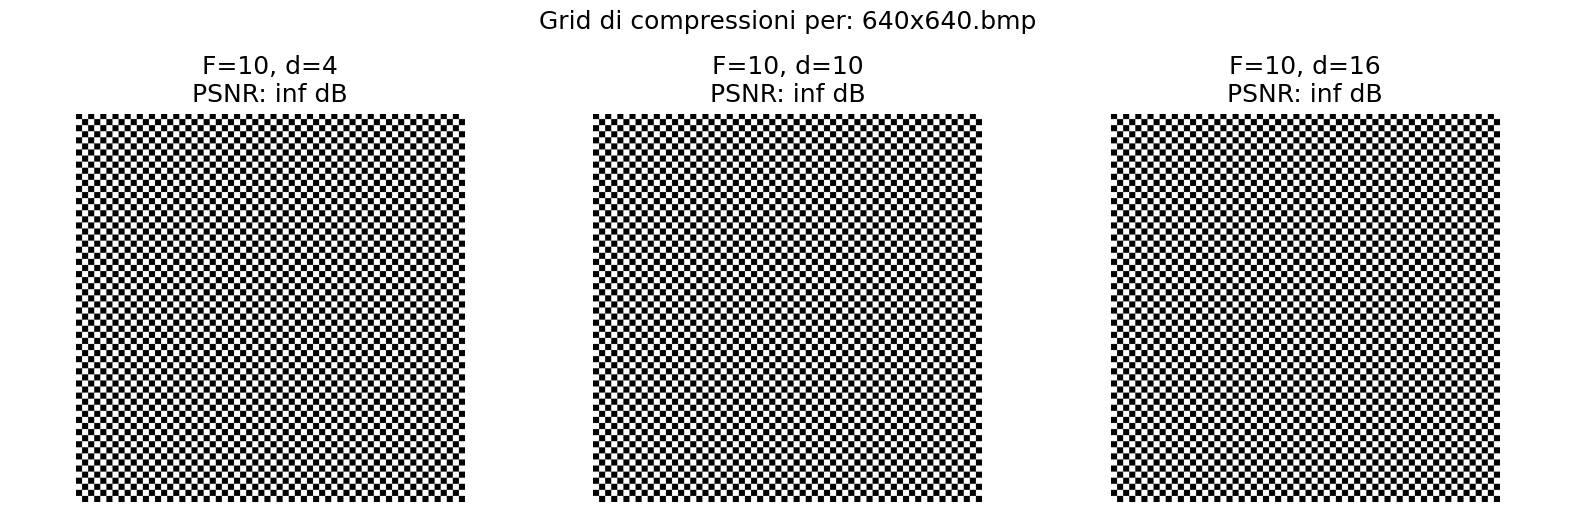
\includegraphics[width=\textwidth,height=0.85\textheight,keepaspectratio]{../relazione/figures/640x640_grid_F10.png}
    \end{figure}
\end{frame}

\begin{frame}{Fotografie Reali: Analisi}
    \begin{itemize}
        \item I casi d'uso reali mostrano un mix di texture naturali, gradienti morbidi e bordi netti.
        \item La comprimibilità complessiva è nettamente superiore alla scacchiera pur rimanendo inferiore al gradiente.
        \item Le immagini naturali risultano intrinsecamente lisce qualora vengano analizzate su piccole aree.
        \item All'interno del singolo blocco l'energia tende a concentrarsi quasi interamente a bassa frequenza.
    \end{itemize}
\end{frame}

\begin{frame}{Fotografie Reali: Risultati}
    \begin{itemize}
        \item Mantenendo appena il $5\%$ dei coefficienti ($d=2$) il PSNR si attesta oltre $28$~dB garantendo una ricostruzione fedele.
        \item Le immagini dotate di vaste superfici uniformi come \texttt{cathedral} si rivelano le più facilmente comprimibili.
        \item Le immagini ricche di texture come \texttt{shoe} generano alte frequenze sparse migliorando rapidamente al crescere di $d$.
        \item A parità di coefficienti i blocchi ampi da $F=32$ catturano dipendenze spaziali più estese comportandosi meglio dei blocchi piccoli.
    \end{itemize}
\end{frame}

\begin{frame}{Ponte: Originale}
    \begin{figure}
        \centering
        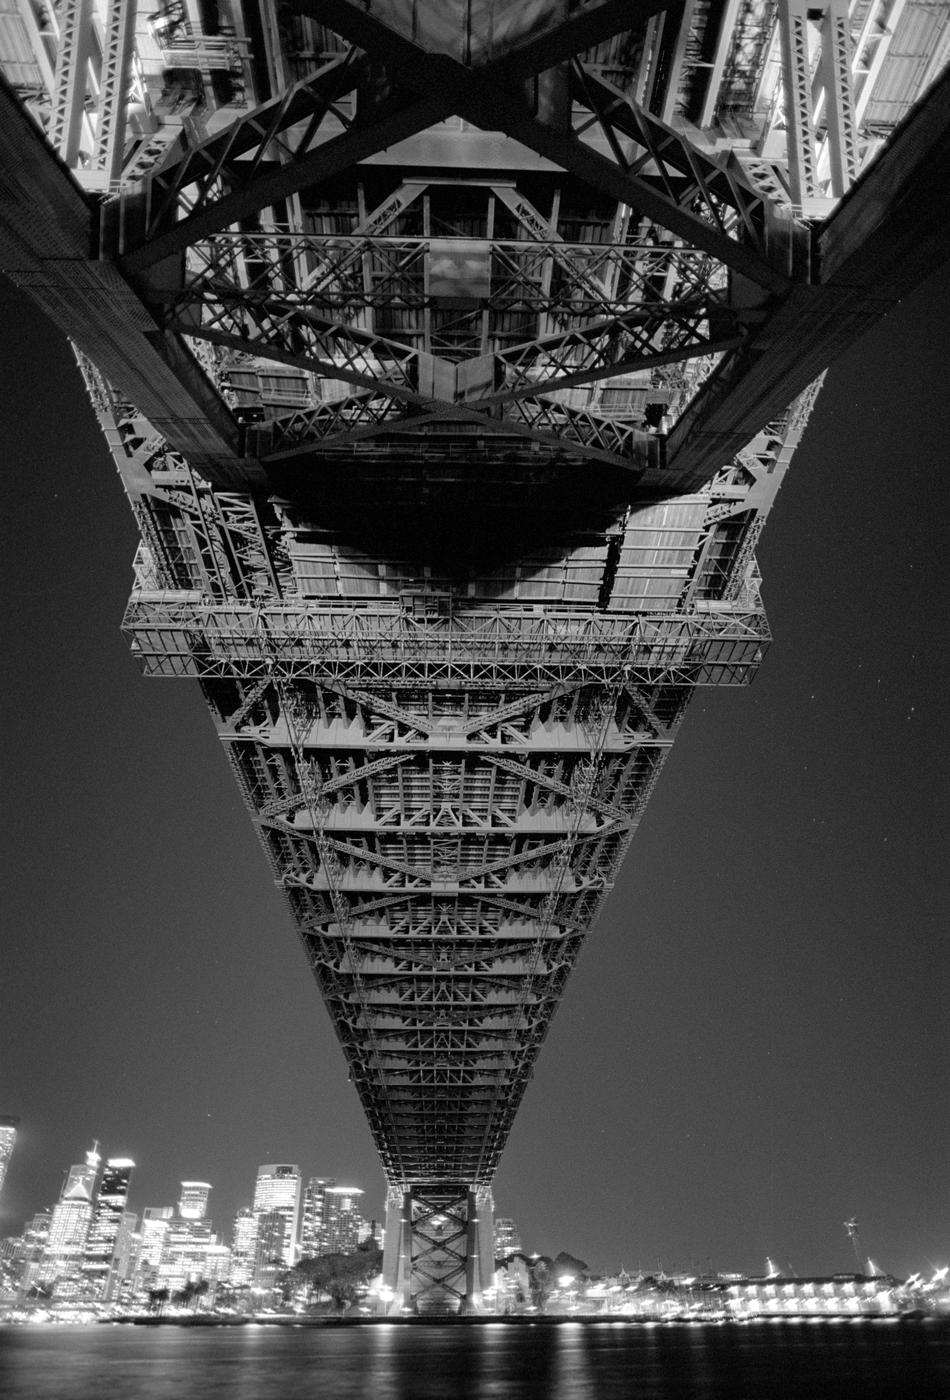
\includegraphics[width=\textwidth,height=0.85\textheight,keepaspectratio]{../relazione/figures/orig_bridge.png}
    \end{figure}
\end{frame}

\begin{frame}{Ponte: Effetti della compressione}
    \begin{figure}
        \centering
        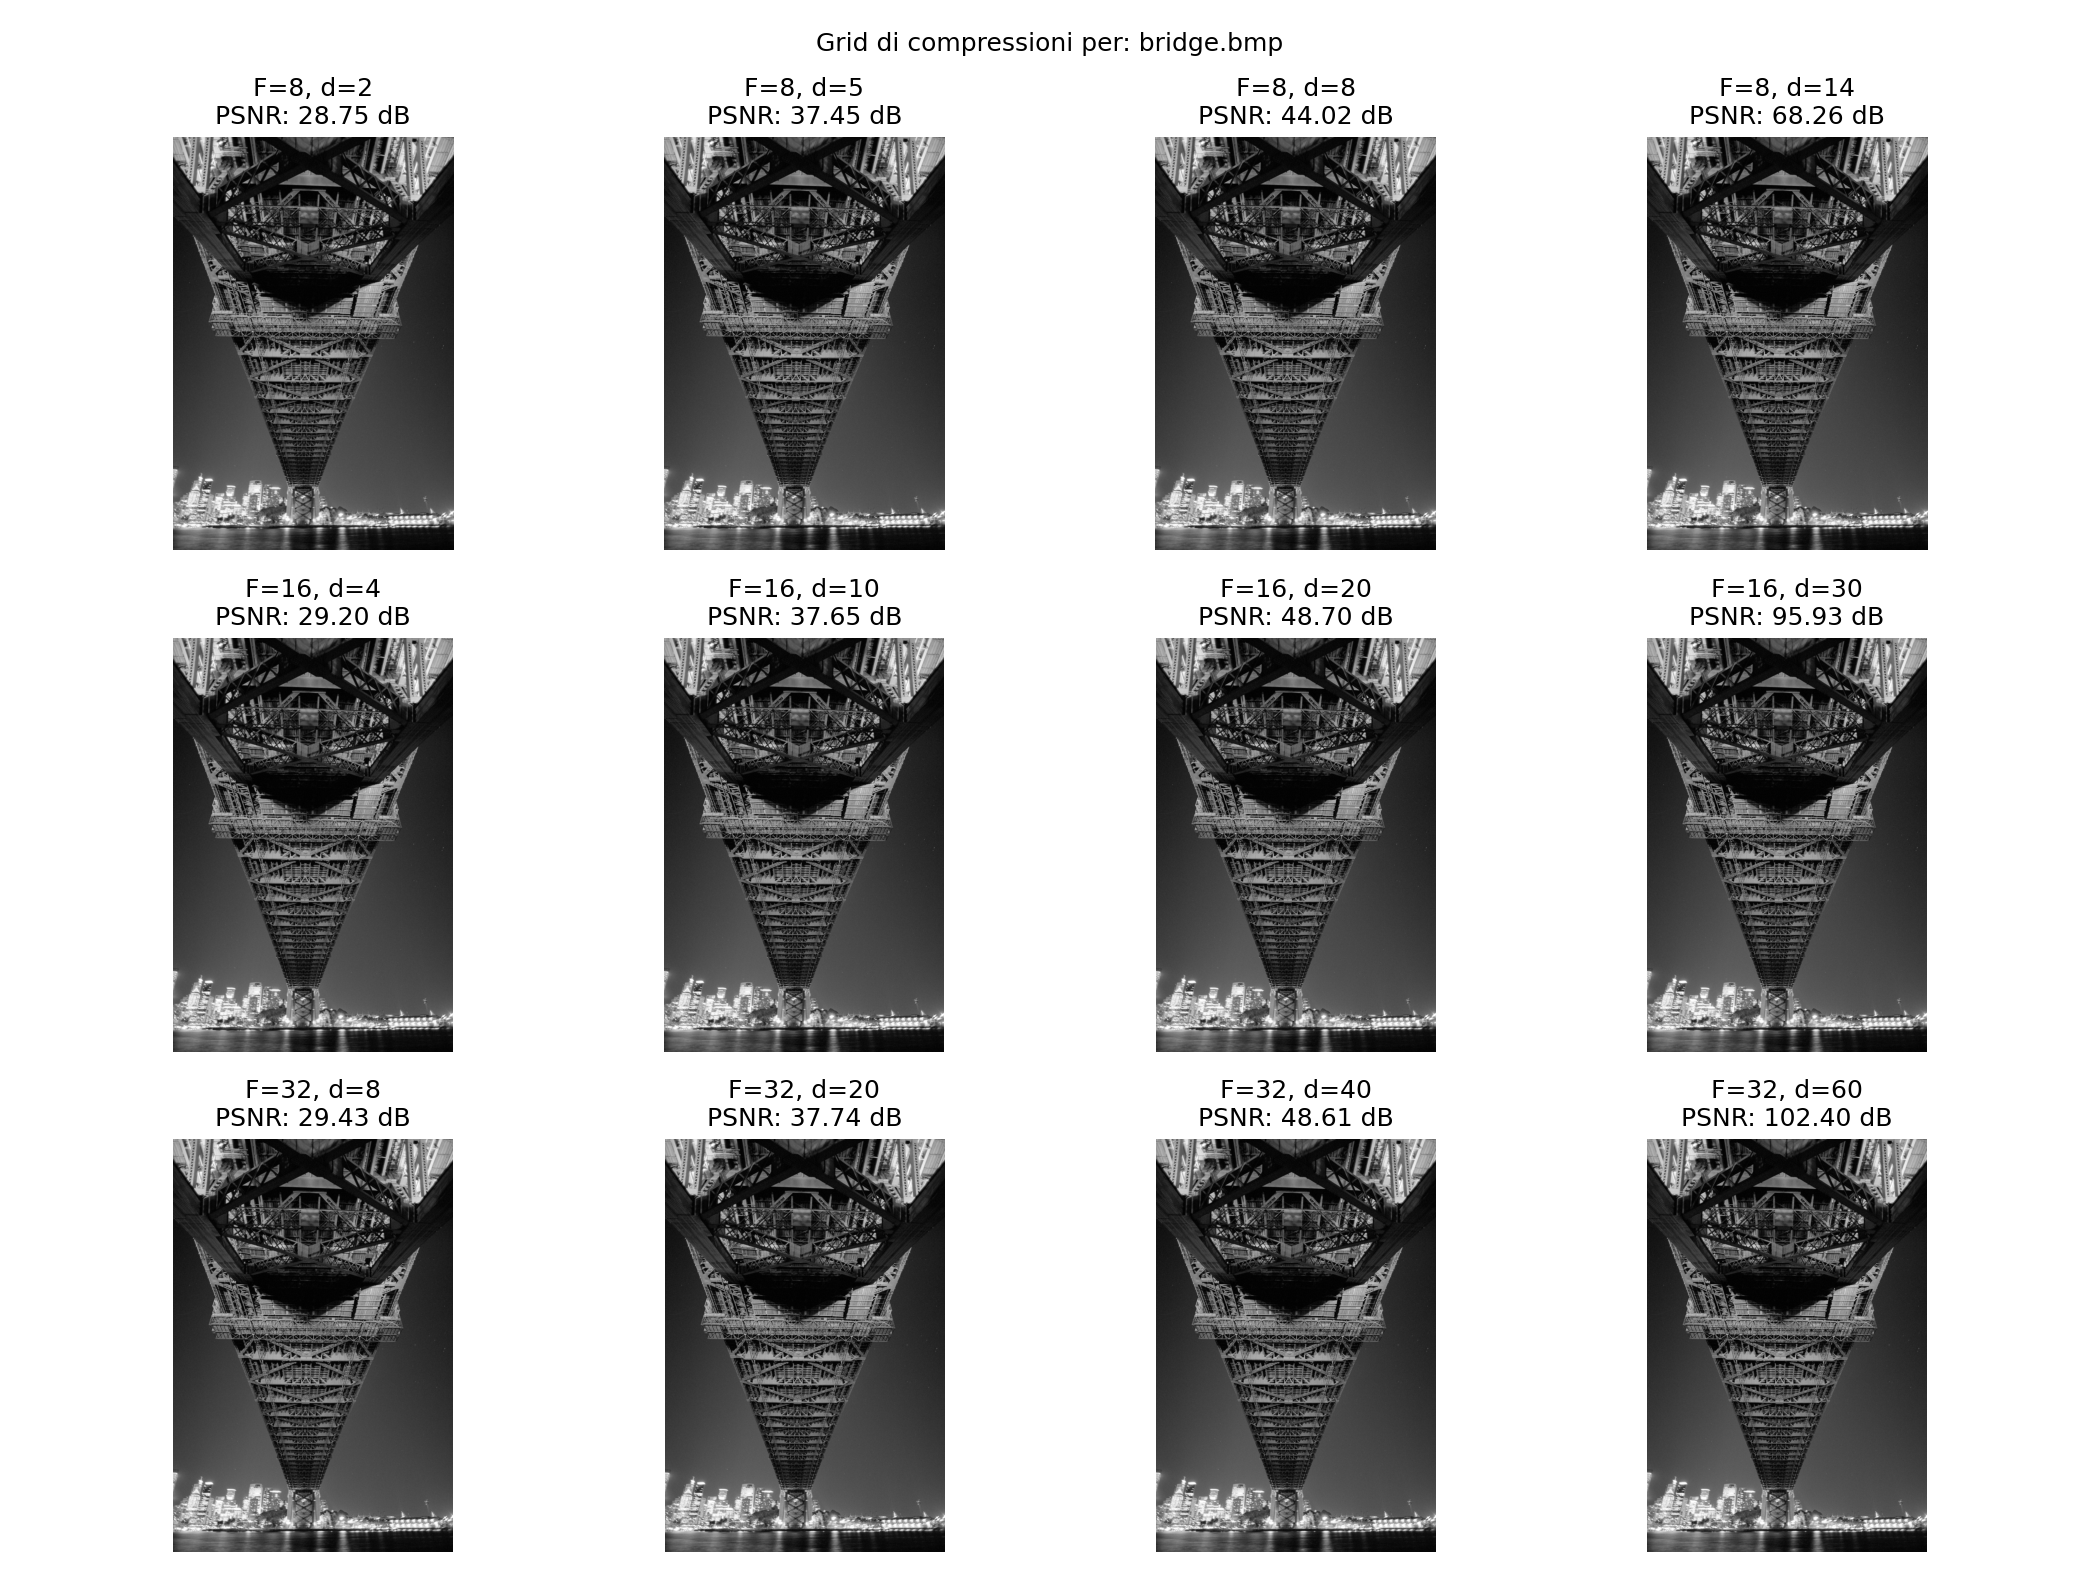
\includegraphics[width=\textwidth,height=0.85\textheight,keepaspectratio]{../relazione/figures/bridge_grid.png}
    \end{figure}
\end{frame}

\begin{frame}{Ponte: PSNR e Metriche}
    \begin{figure}
        \centering
        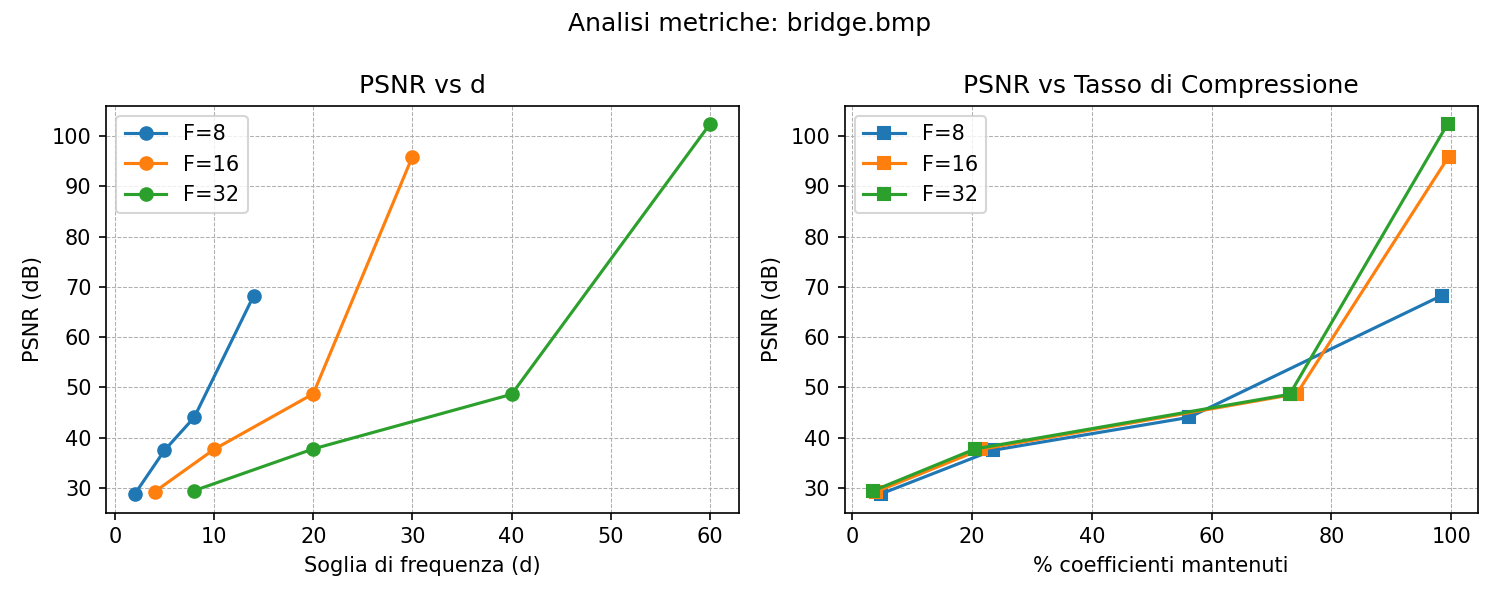
\includegraphics[width=\textwidth,height=0.85\textheight,keepaspectratio]{../relazione/figures/bridge_metrics.png}
    \end{figure}
\end{frame}

\begin{frame}{Cattedrale: Originale}
    \begin{figure}
        \centering
        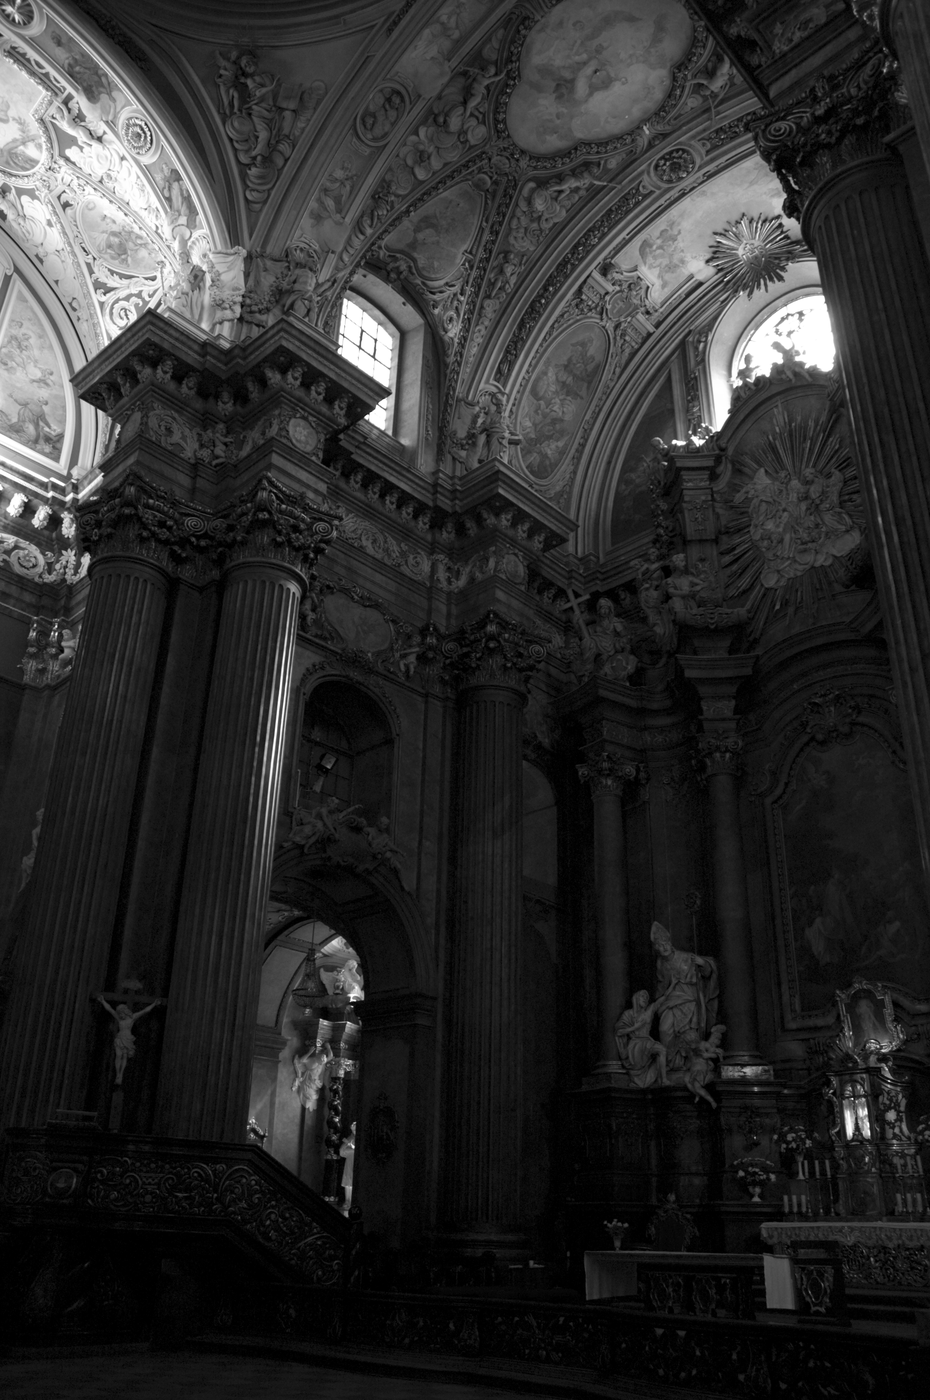
\includegraphics[width=\textwidth,height=0.85\textheight,keepaspectratio]{../relazione/figures/orig_cathedral.png}
    \end{figure}
\end{frame}

\begin{frame}{Cattedrale:Effetti della compressione}
    \begin{figure}
        \centering
        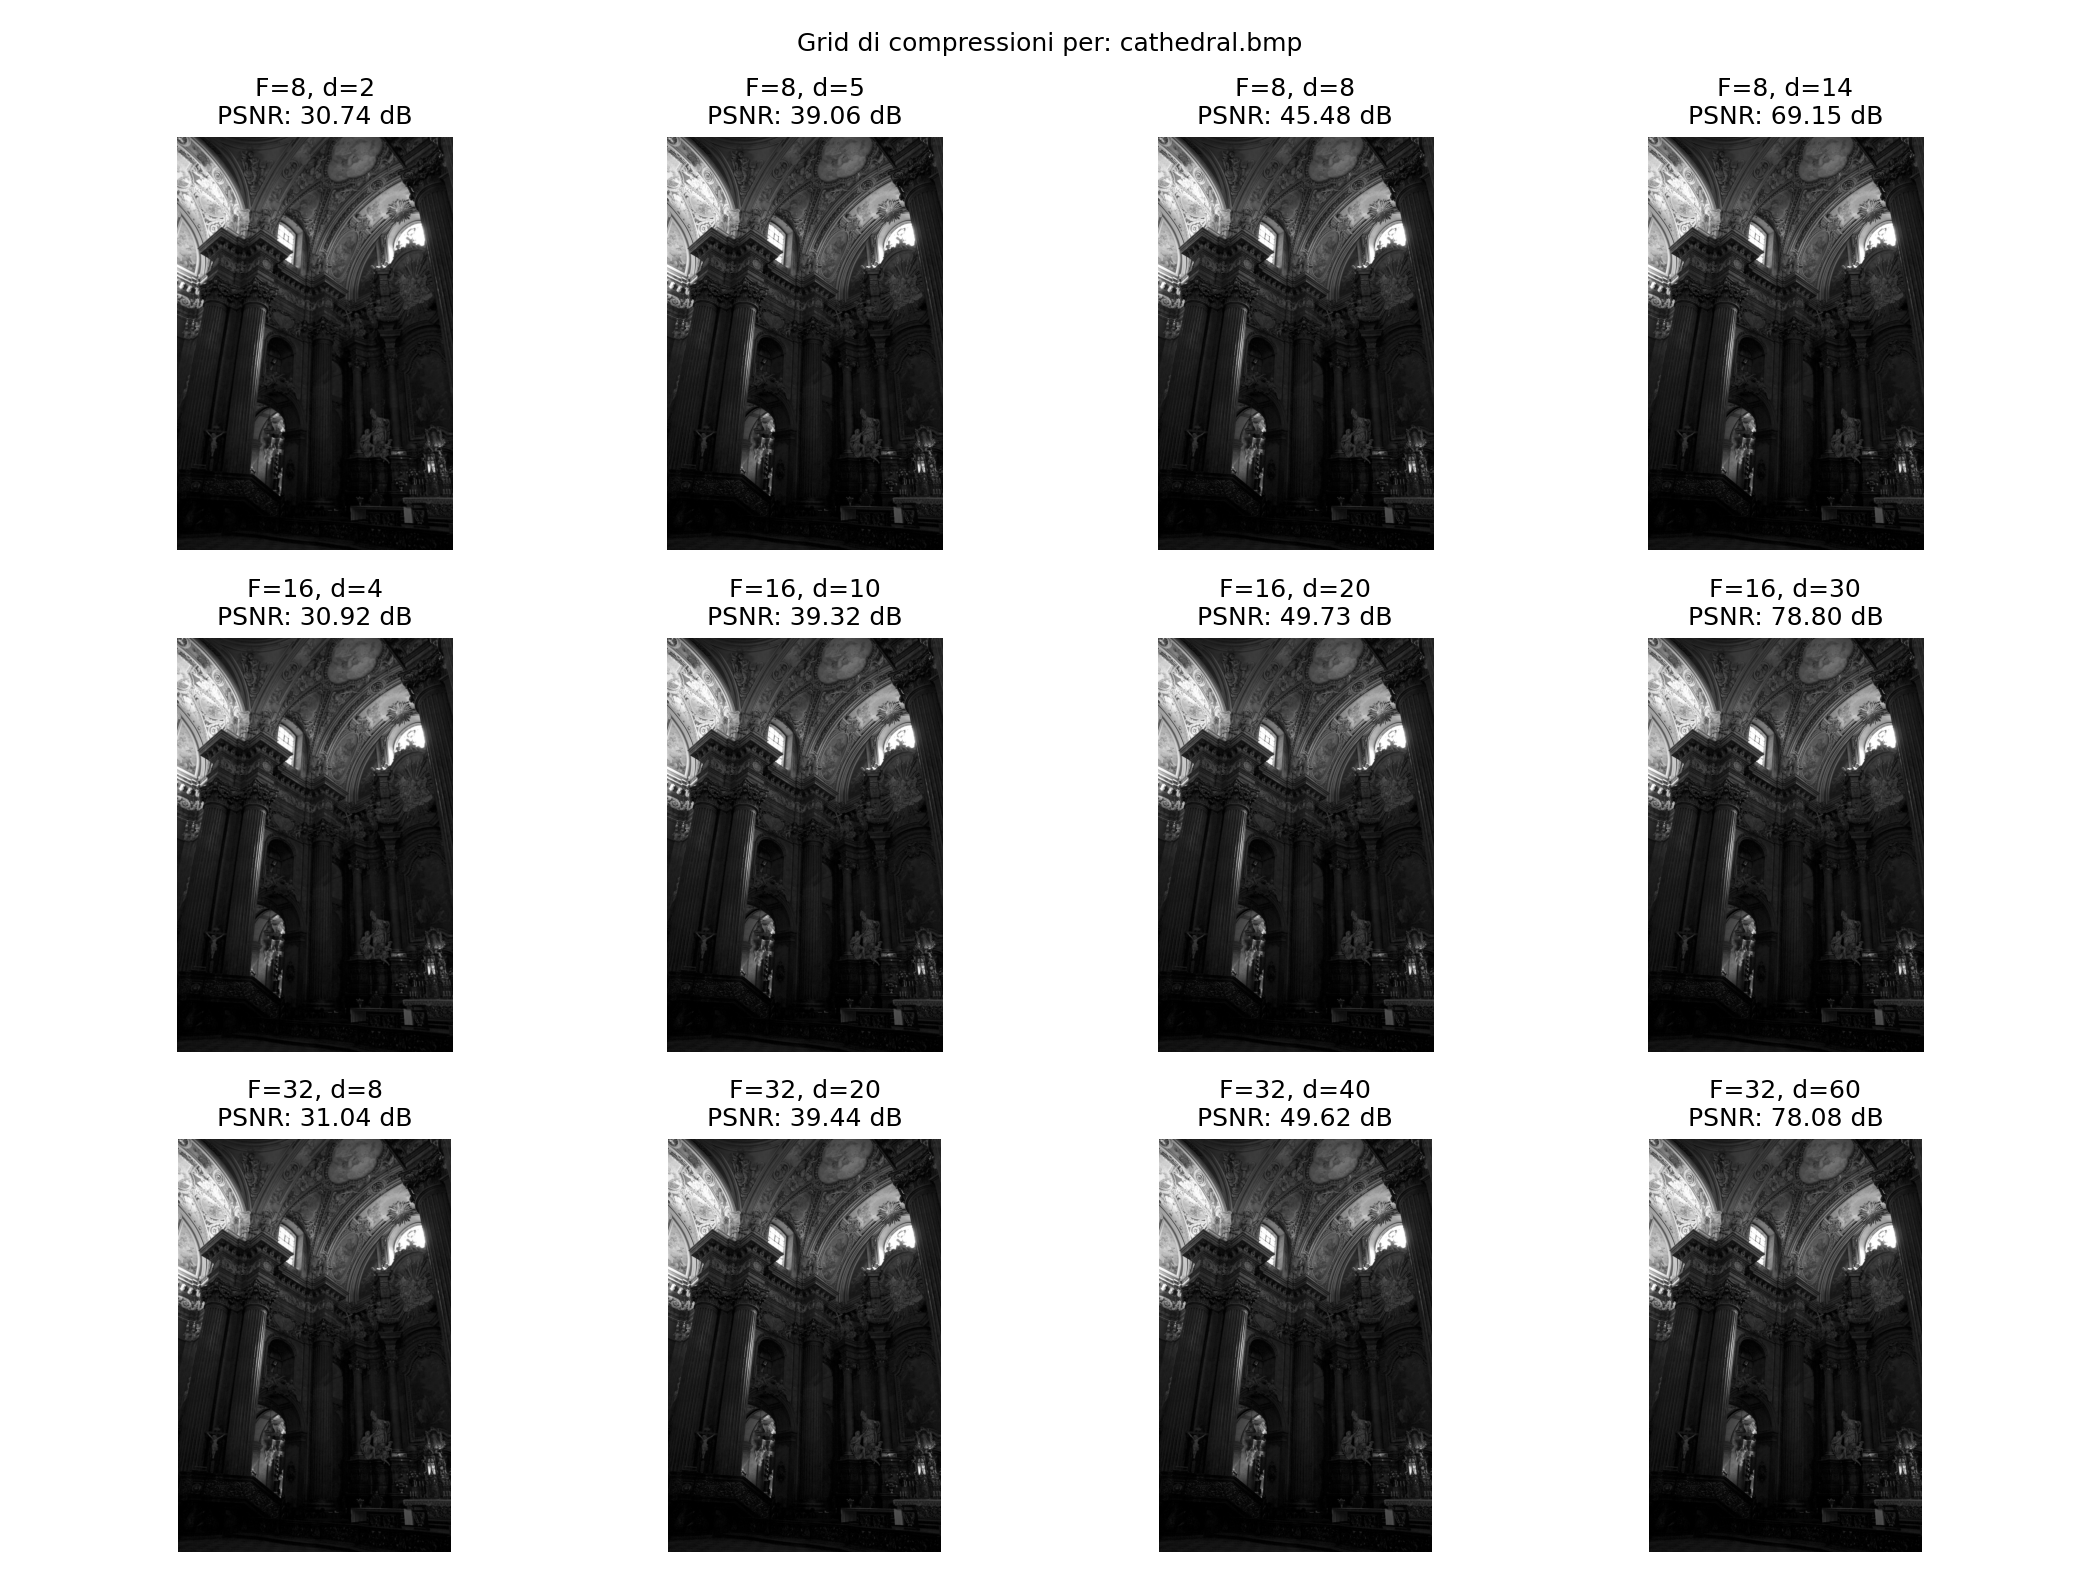
\includegraphics[width=\textwidth,height=0.85\textheight,keepaspectratio]{../relazione/figures/cathedral_grid.png}
    \end{figure}
\end{frame}

\begin{frame}{Cattedrale: PSNR e Metriche}
    \begin{figure}
        \centering
        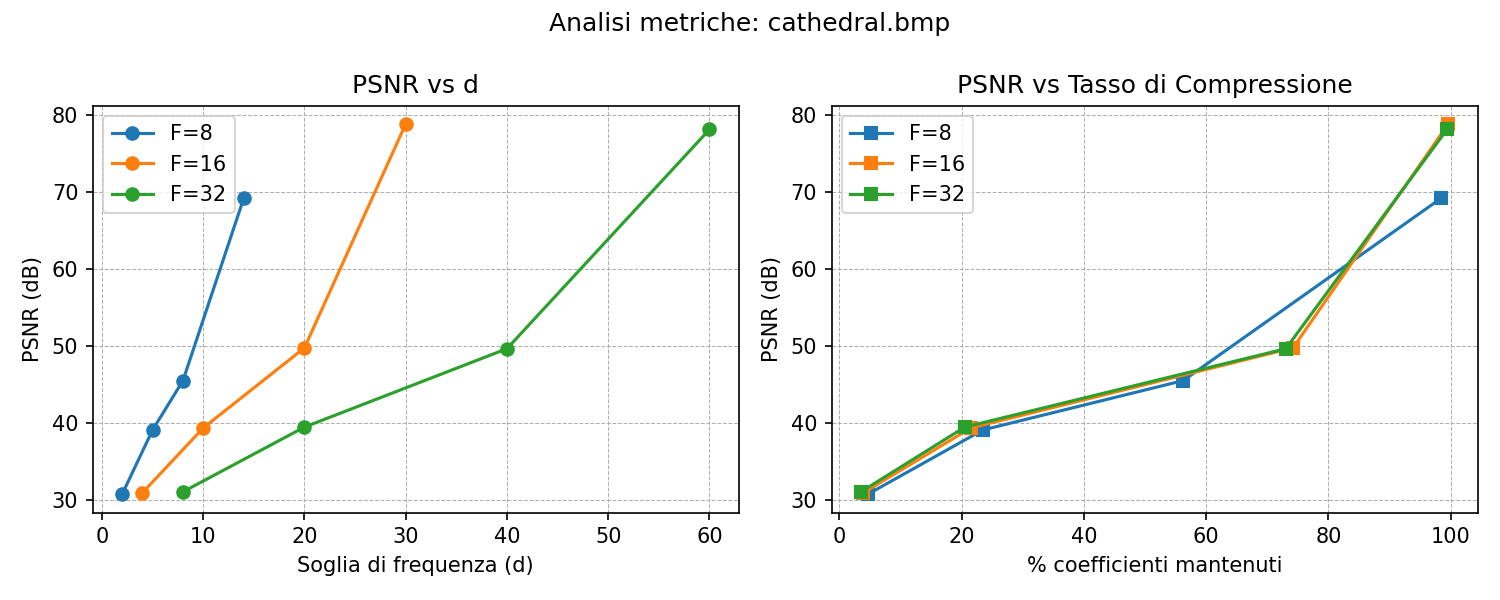
\includegraphics[width=\textwidth,height=0.85\textheight,keepaspectratio]{../relazione/figures/cathedral_metrics.png}
    \end{figure}
\end{frame}

\begin{frame}{Cervo: Originale}
    \begin{figure}
        \centering
        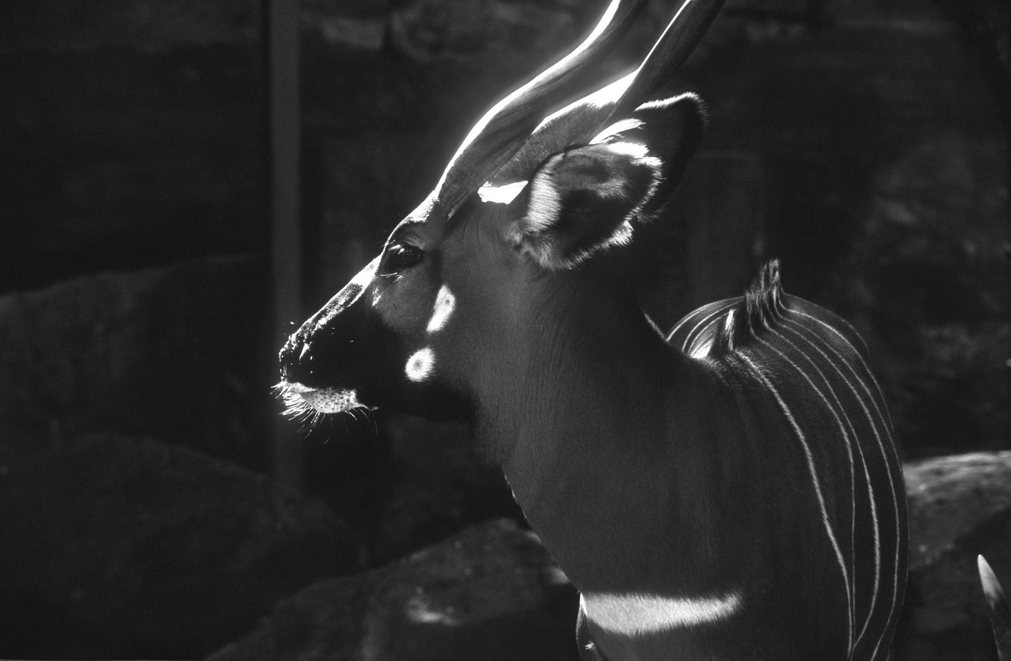
\includegraphics[width=\textwidth,height=0.85\textheight,keepaspectratio]{../relazione/figures/orig_deer.png}
    \end{figure}
\end{frame}

\begin{frame}{Cervo: Effetti della compressione}
    \begin{figure}
        \centering
        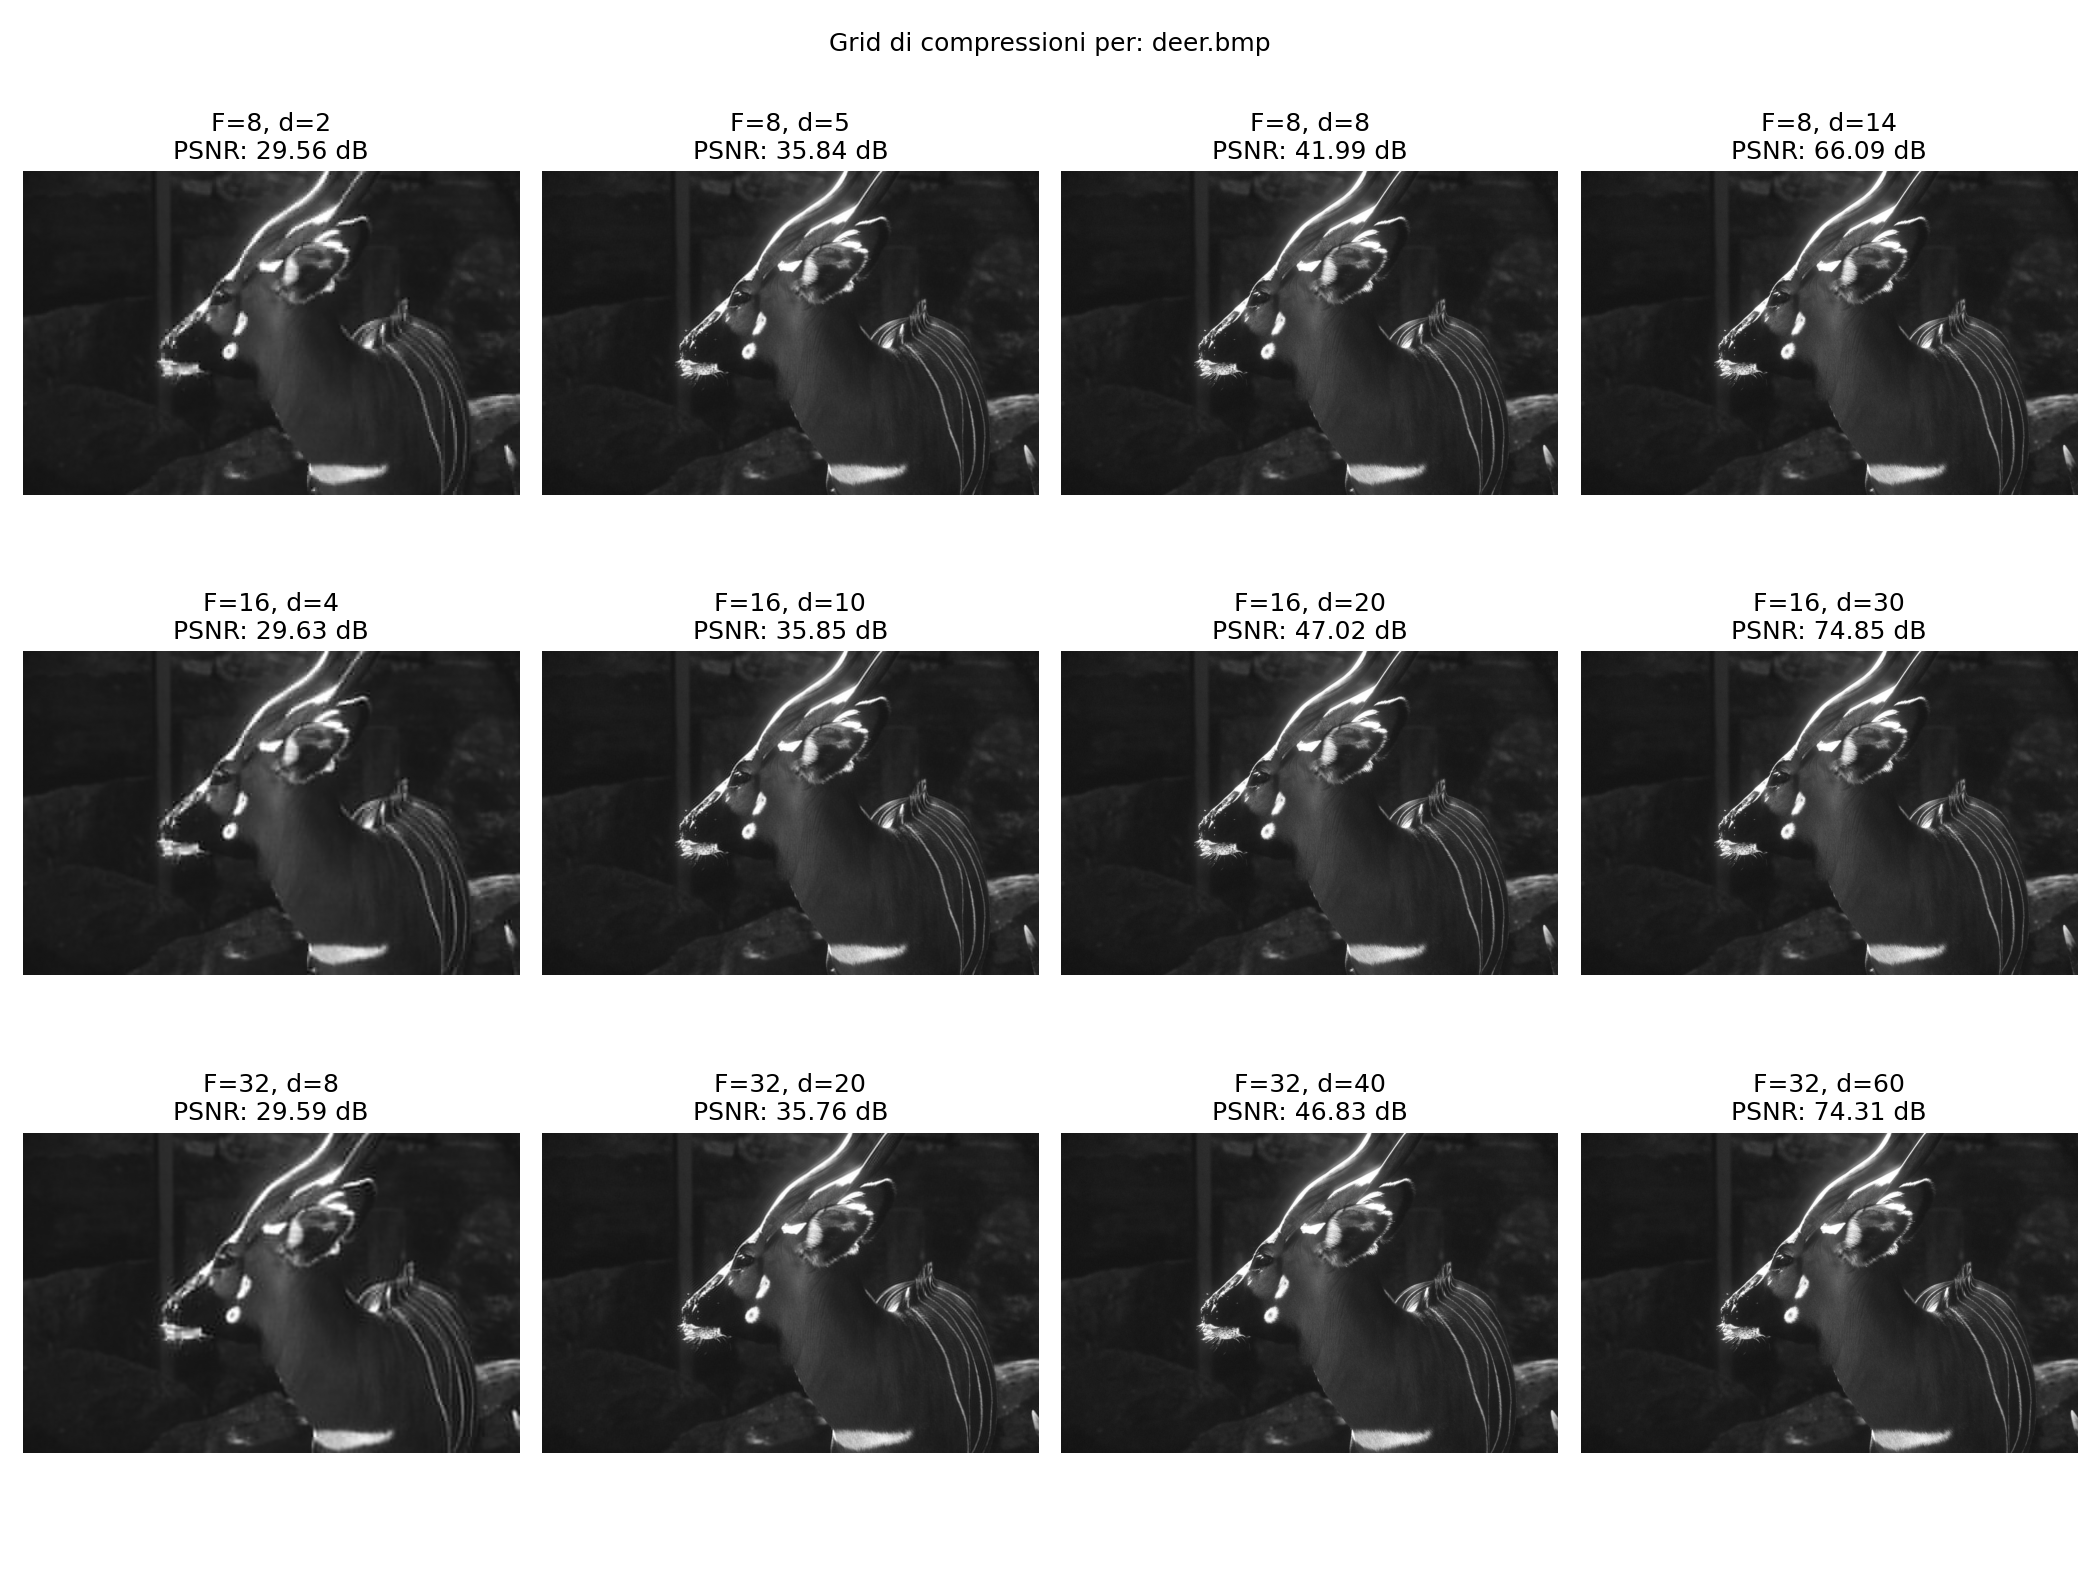
\includegraphics[width=\textwidth,height=0.85\textheight,keepaspectratio]{../relazione/figures/deer_grid.png}
    \end{figure}
\end{frame}

\begin{frame}{Cervo: PSNR e Metriche}
    \begin{figure}
        \centering
        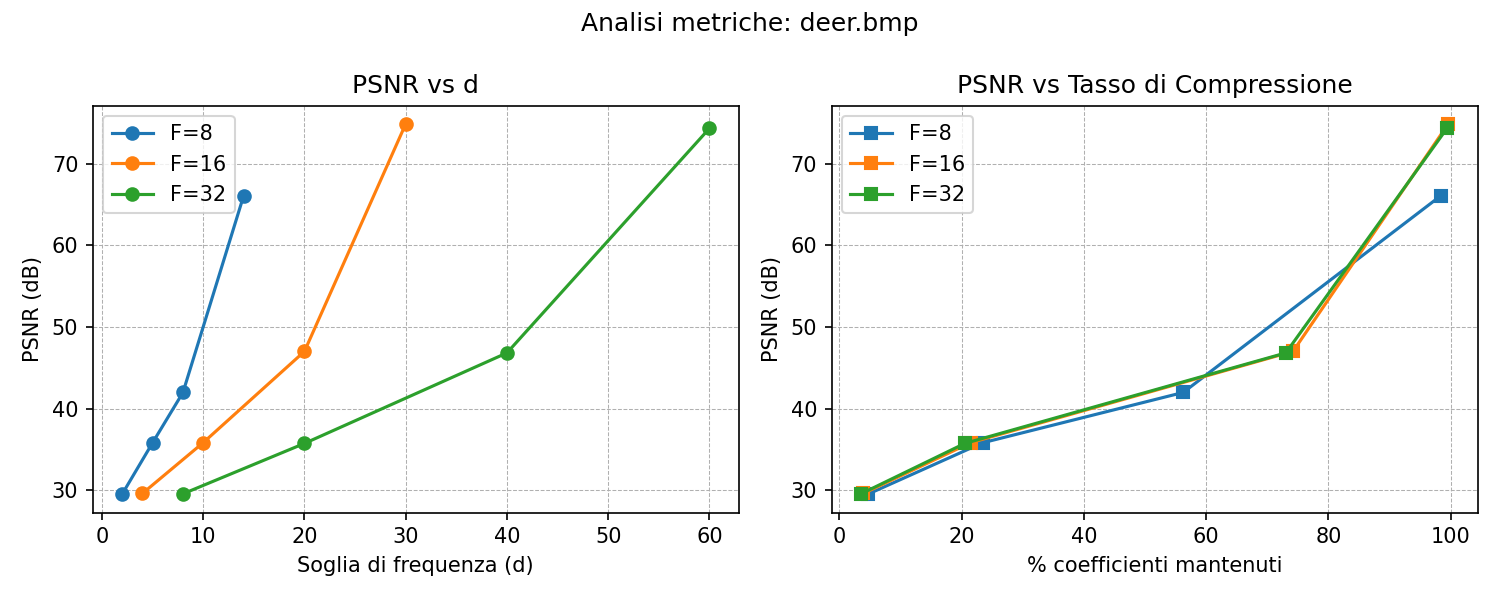
\includegraphics[width=\textwidth,height=0.85\textheight,keepaspectratio]{../relazione/figures/deer_metrics.png}
    \end{figure}
\end{frame}

\begin{frame}{Scarpa: Originale}
    \begin{figure}
        \centering
        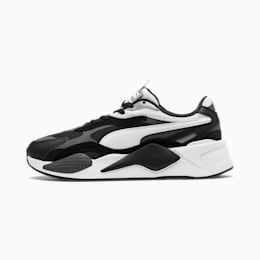
\includegraphics[width=\textwidth,height=0.85\textheight,keepaspectratio]{../relazione/figures/orig_shoe.png}
    \end{figure}
\end{frame}

\begin{frame}{Scarpa: Effetti della compressione}
    \begin{figure}
        \centering
        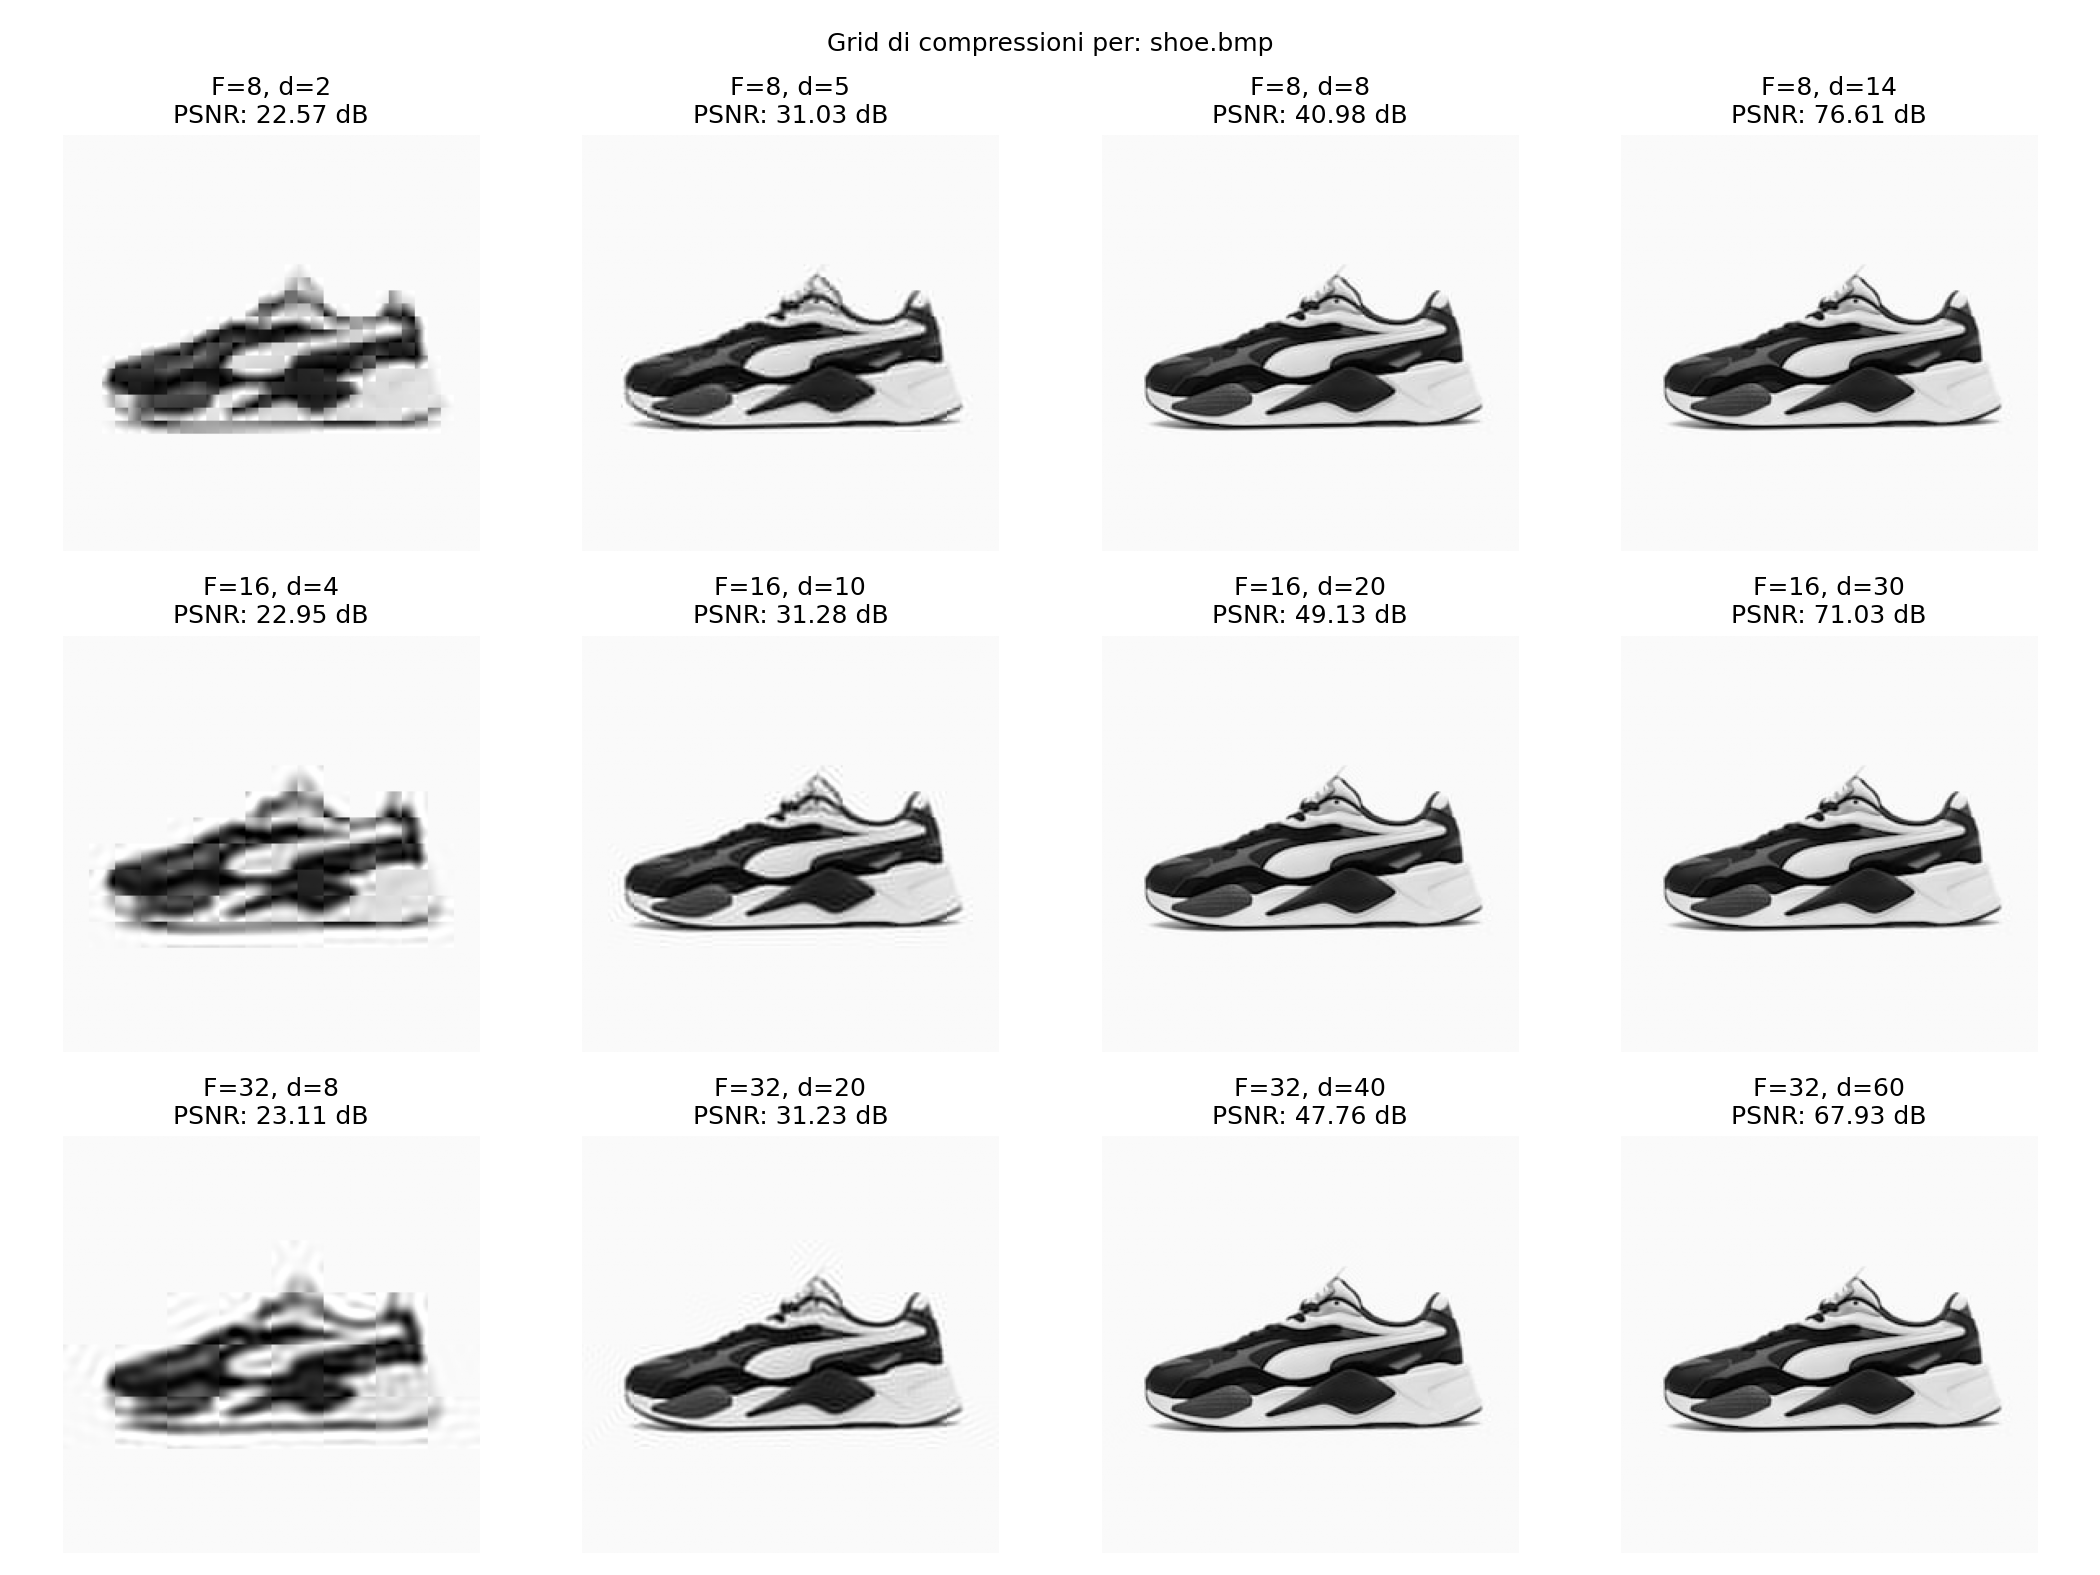
\includegraphics[width=\textwidth,height=0.85\textheight,keepaspectratio]{../relazione/figures/shoe_grid.png}
    \end{figure}
\end{frame}

\begin{frame}{Scarpa: PSNR e Metriche}
    \begin{figure}
        \centering
        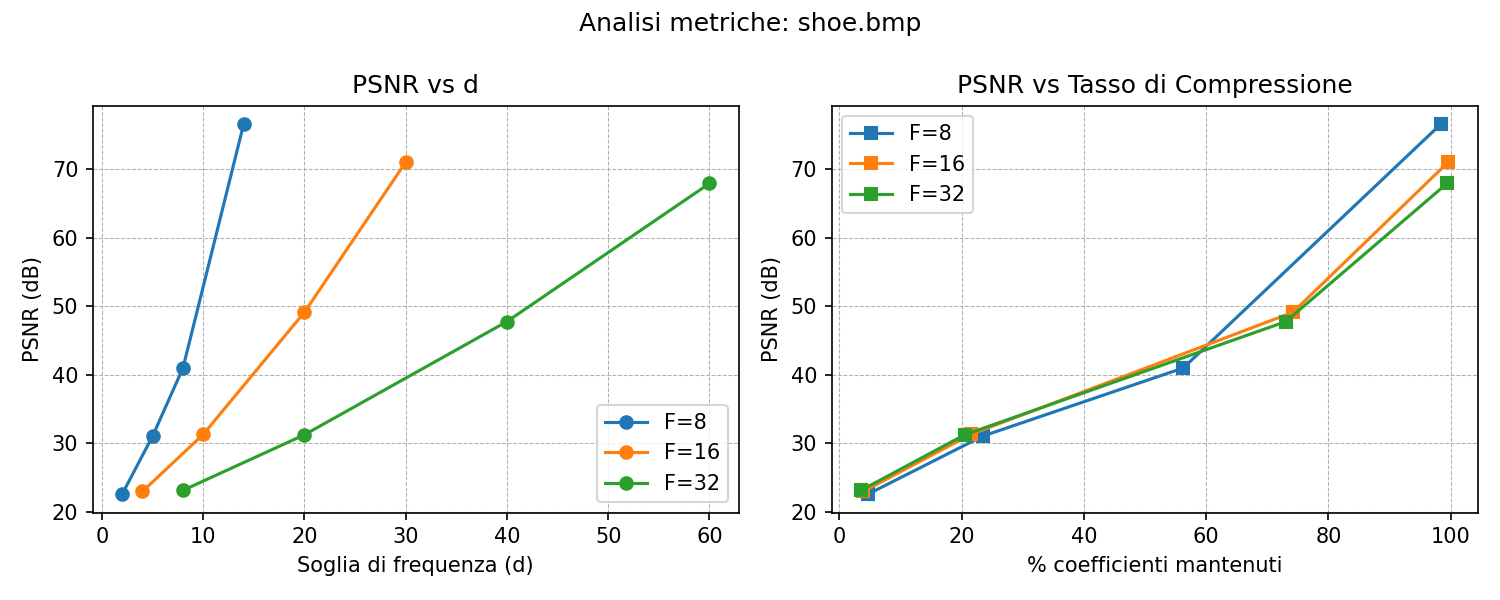
\includegraphics[width=\textwidth,height=0.85\textheight,keepaspectratio]{../relazione/figures/shoe_metrics.png}
    \end{figure}
\end{frame}

\begin{frame}{Tony Pitony: Originale}
    \begin{figure}
        \centering
        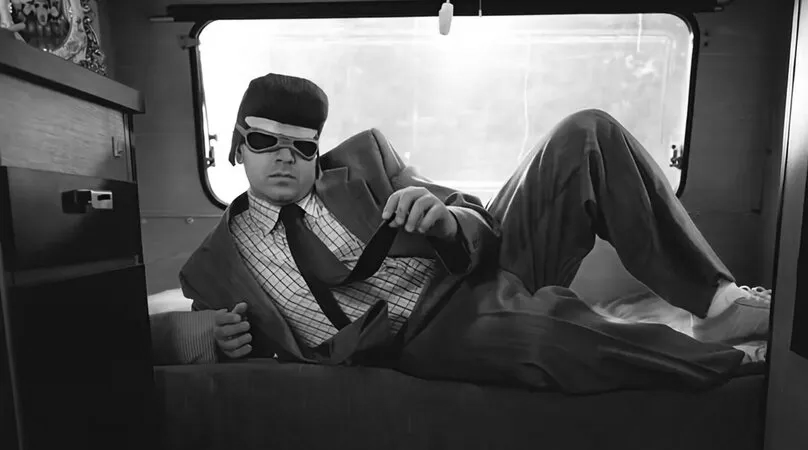
\includegraphics[width=\textwidth,height=0.85\textheight,keepaspectratio]{../relazione/figures/orig_tonypitony.png}
    \end{figure}
\end{frame}

\begin{frame}{Tony Pitony: Effetti della compressione}
    \begin{figure}
        \centering
        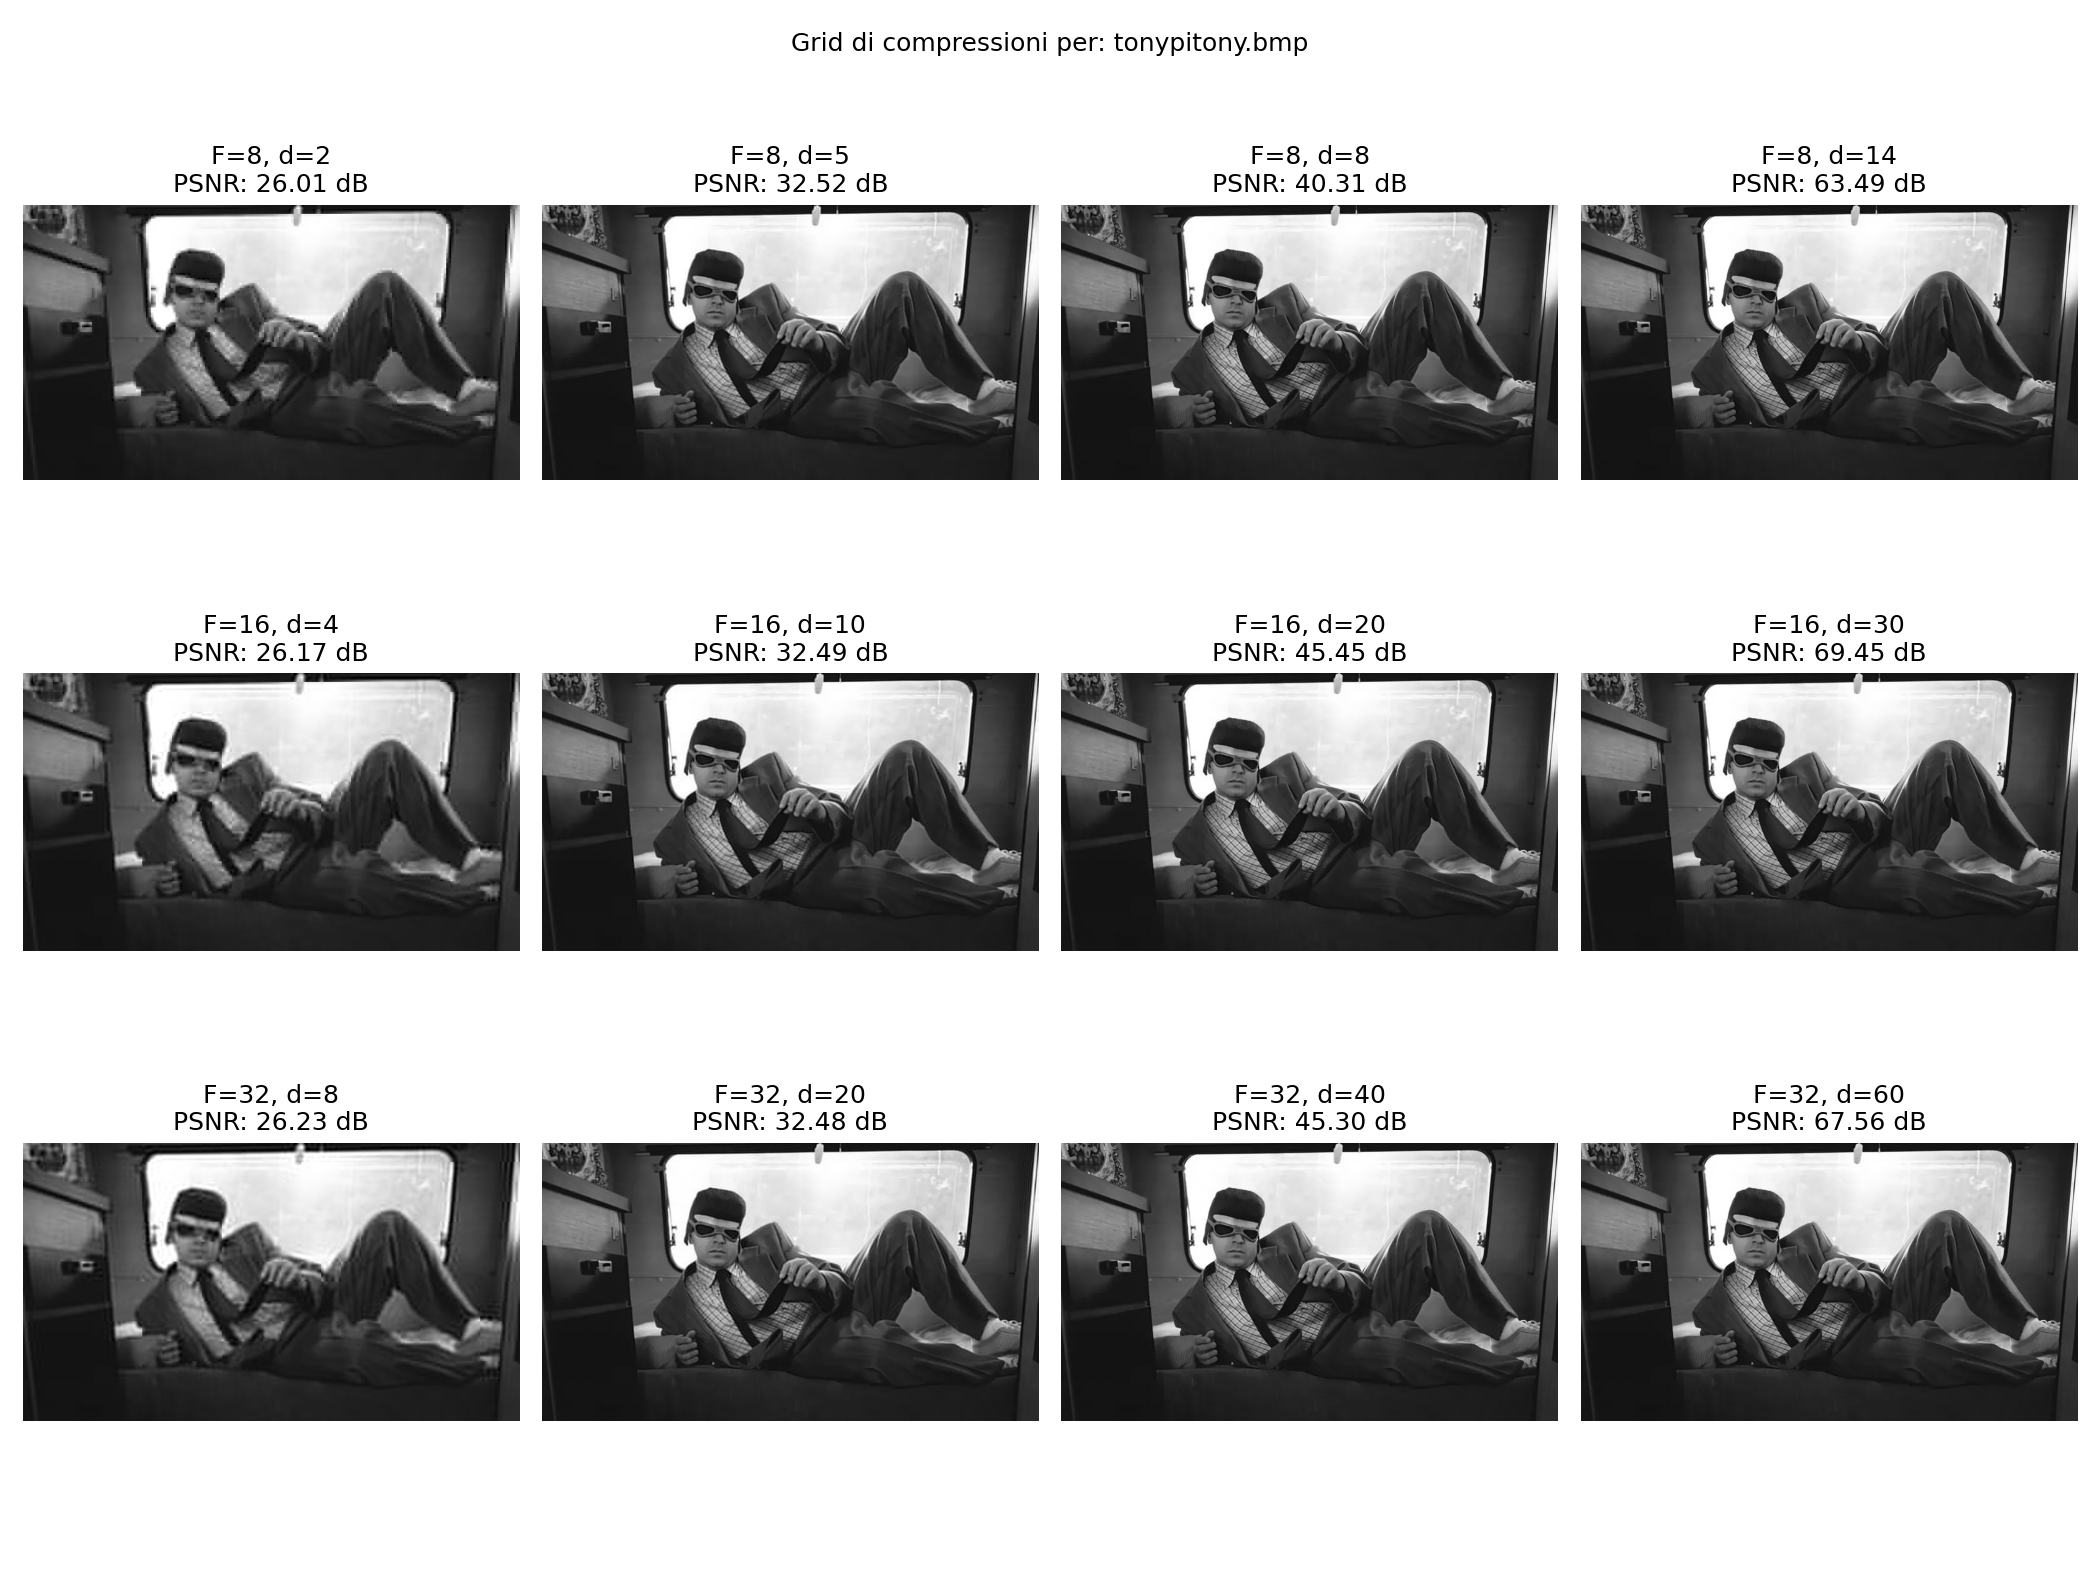
\includegraphics[width=\textwidth,height=0.85\textheight,keepaspectratio]{../relazione/figures/tonypitony_grid.png}
    \end{figure}
\end{frame}

\begin{frame}{Tony Pitony: PSNR e Metriche}
    \begin{figure}
        \centering
        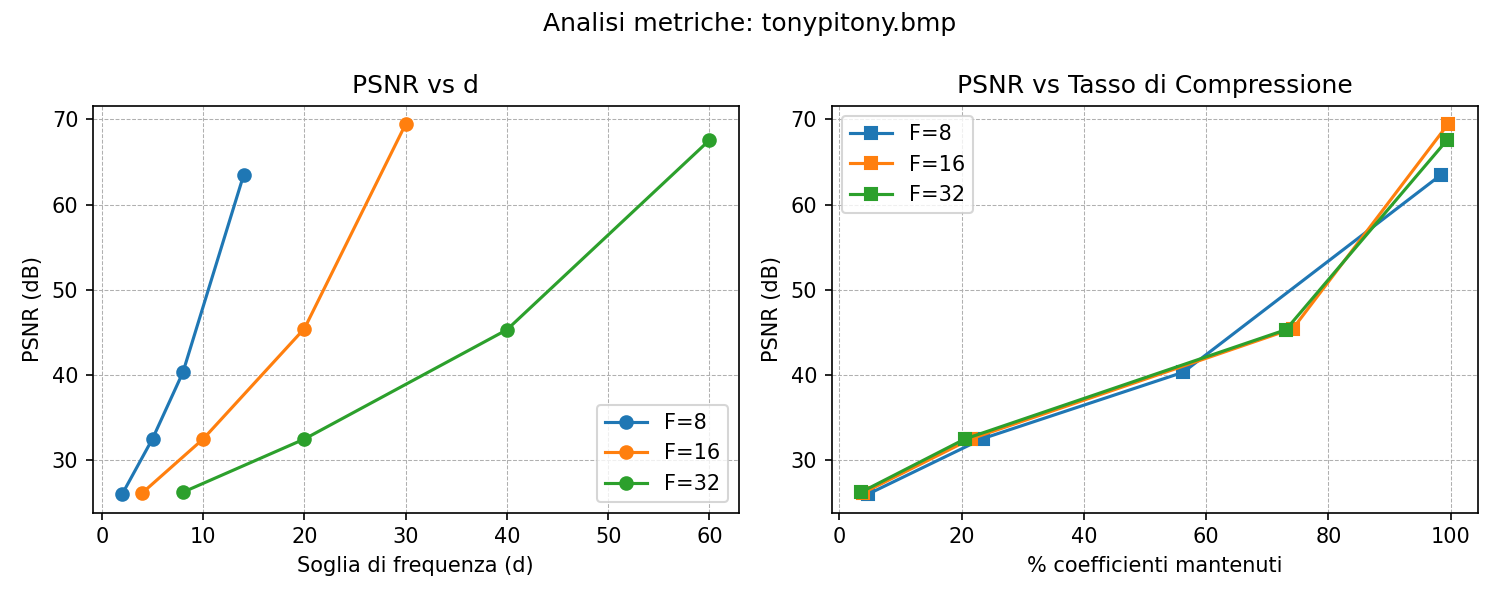
\includegraphics[width=\textwidth,height=0.85\textheight,keepaspectratio]{../relazione/figures/tonypitony_metrics.png}
    \end{figure}
\end{frame}

\begin{frame}[plain]
    \begin{center}
        \Huge{Grazie per l'attenzione}
    \end{center}
\end{frame}

\end{document}
